\documentclass{article}

\usepackage{a4wide}
\usepackage[T1]{fontenc}
\usepackage{textcomp}
\usepackage[utf8]{inputenc}
\usepackage[french]{babel}
\usepackage[babel=true]{csquotes} 
\usepackage[export]{adjustbox}% http://ctan.org/pkg/adjustbox
\usepackage{graphicx}
\graphicspath{{image/}}
\usepackage{amsmath}
\usepackage{color}
\usepackage{hyperref}
\usepackage[section]{placeins}


\hypersetup{colorlinks,linkcolor=,urlcolor=blue}


\title{Sécurité Informatique - CC1}
\author{Fr\'ed\'erick Fabre Ferber , M1 Informatique}
\begin{document}

\maketitle


\begin{abstract}
Ce rapport résume le travail fait dans le cadre du cours de Sécurité Informatique. Il consiste en l'élaboration de différents algorithmes de chiffrement via Android Studio.
Nous présenterons ceux mentionnés ci-dessous :
\begin{itemize}
\item Atbash
\item César
\item Vigenère
\item Playfair
\item Hill
\item Transposition Rectangulaire
\item DES
\item Un algorithme surprise
\item L'algorithme RSA 
\end{itemize}
\end{abstract}


\section{Fonctionnement de l'application}

L'application Android pour ce projet est composé de deux activités : 
\begin{itemize}
\item \textbf{MainActivity} qui consiste tout simplement en l'affichage d'une liste contenant tous les algorithmes de chiffrement via une \textbf{ListView}. Quand on clique sur un des éléments, on envoie son id et son nom à l'activité \textbf{CryptoDefaultActivity} avec un \textbf{Intent} \textbf{(voir figure  \ref{fig:main})}.
\vspace{1\baselineskip}

\item \textbf{CryptoDefaultActivity}, c'est elle qui gère le chiffrement et le déchiffrement pour chaque algorithme. Elle se compose de 3 champs (\textbf{\textit{Message clair}, \textit{Message chiffré} et \textit{clé}}). 
Un autre champ peut se rajouter ou s'enlever en fonction de l'algorithme (ex : Hill,Atbash). L'affichage est géré par le \textbf{layout} \textit{crypto\_default\_layout.xml} \textbf{(voir figure \ref{fig:exemple} et \ref{fig:layout})} .
Quand on appuie sur le bouton chiffrer ou déchiffrer, on va alors modifier le champ \textbf{message chiffré} en sélectionnant l'algorithme correspondant à l'id reçu. Cela nous permet de n'avoir qu'un seul layout et qu'une seule activité pour le chiffrage déchiffrage.

\end{itemize}
\vspace{1\baselineskip}

Aperçu du code : 
\vspace{1\baselineskip}

\begin{verbatim}
if (!(message.isEmpty())){

switch (chiffrementID){

    /* Atbash */
    case 0 :
          messageChiffreEdit.setText(Crypto.atbash(message));
          break;

    /*César 3*/
    case 1 :
		 if(!(cle.isEmpty())){
         int decalage = Integer.parseInt(cle);
         messageChiffreEdit.setText(Crypto.cesar(message , decalage ,chiffre));
         break;
}
    /*Vigenère*/
    case 2 :

      if(!(cle.isEmpty())){ 
       messageChiffreEdit.setText(Crypto.vigenere(message , cle , chiffre));                         
       break;
}
         .....
\end{verbatim}

\begin{figure}[h!]
\centering
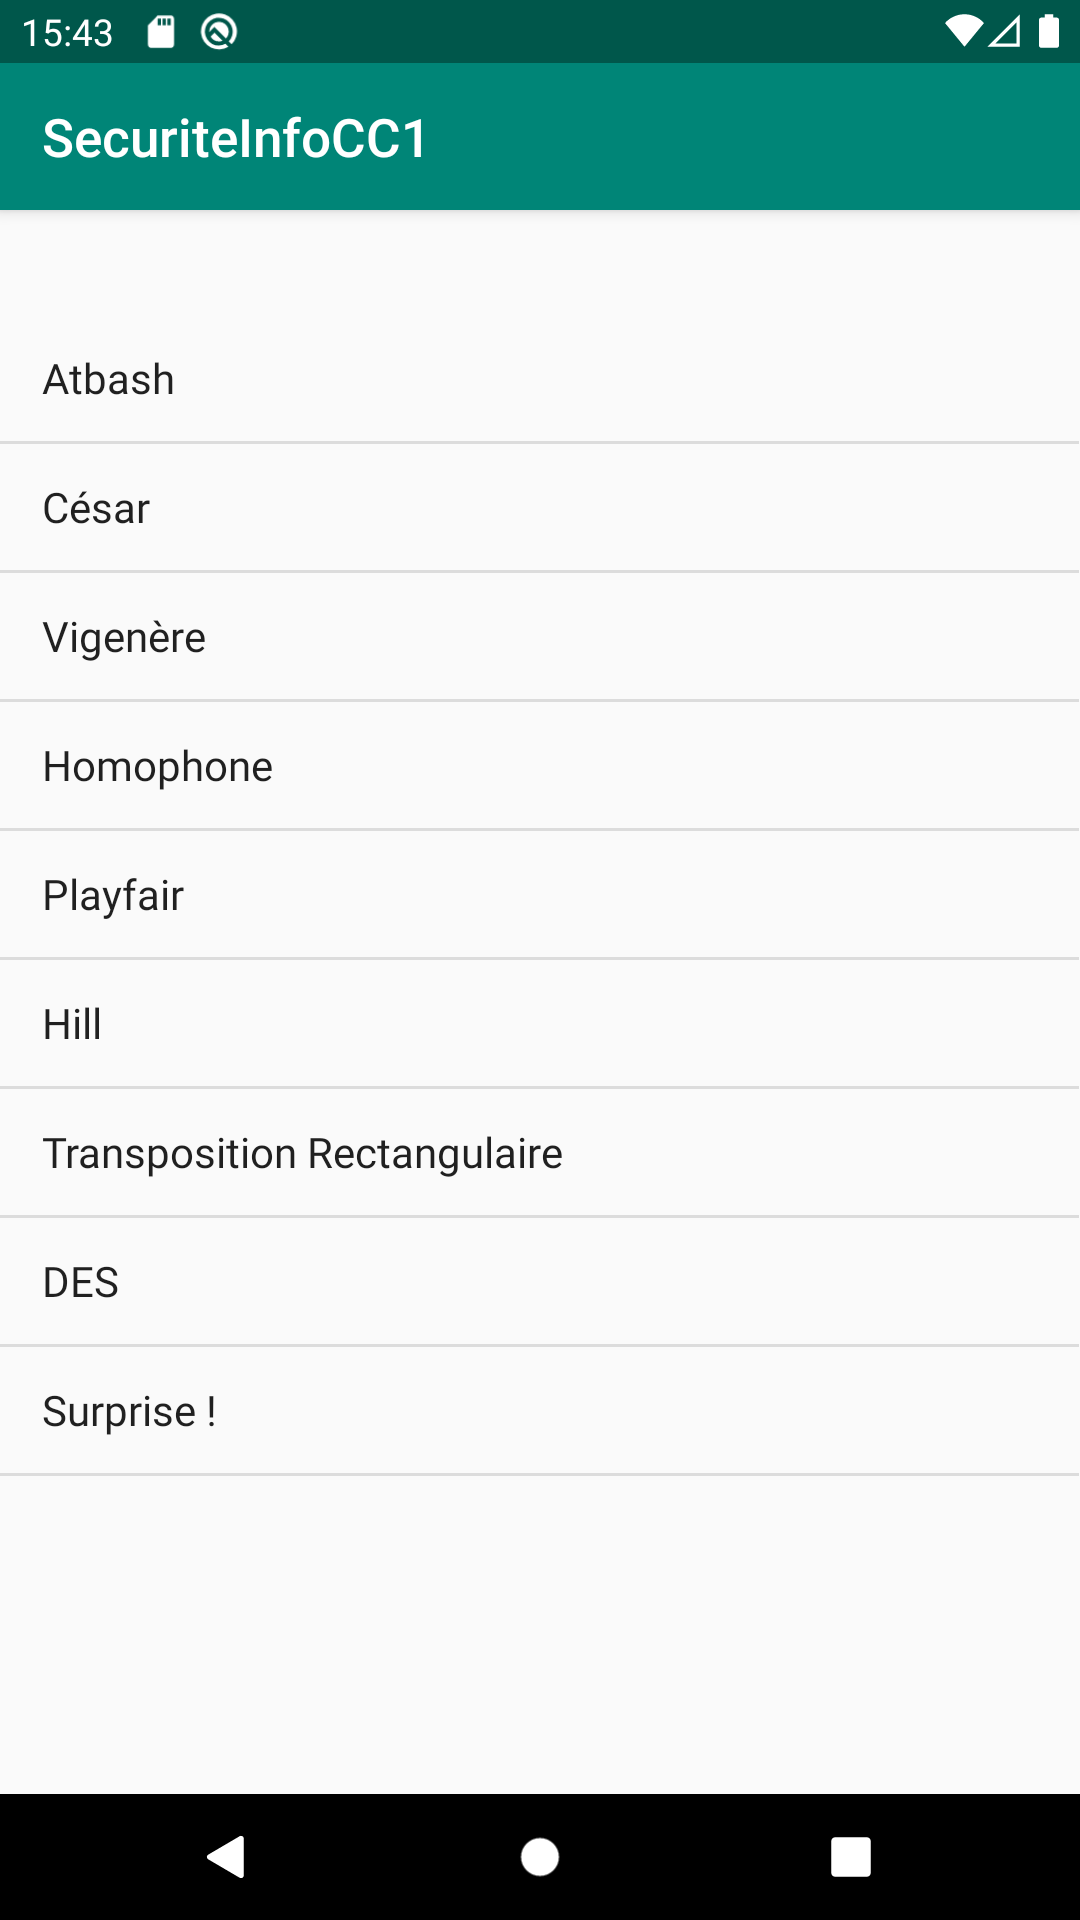
\includegraphics[scale=0.15]{./img/main.png}
\caption{Vue de l'activité principale \textbf{MainActivity} \label{fig:main}}
\end{figure}

\begin{figure}[tb]
    \centering
    \begin{tabular}{cc}
      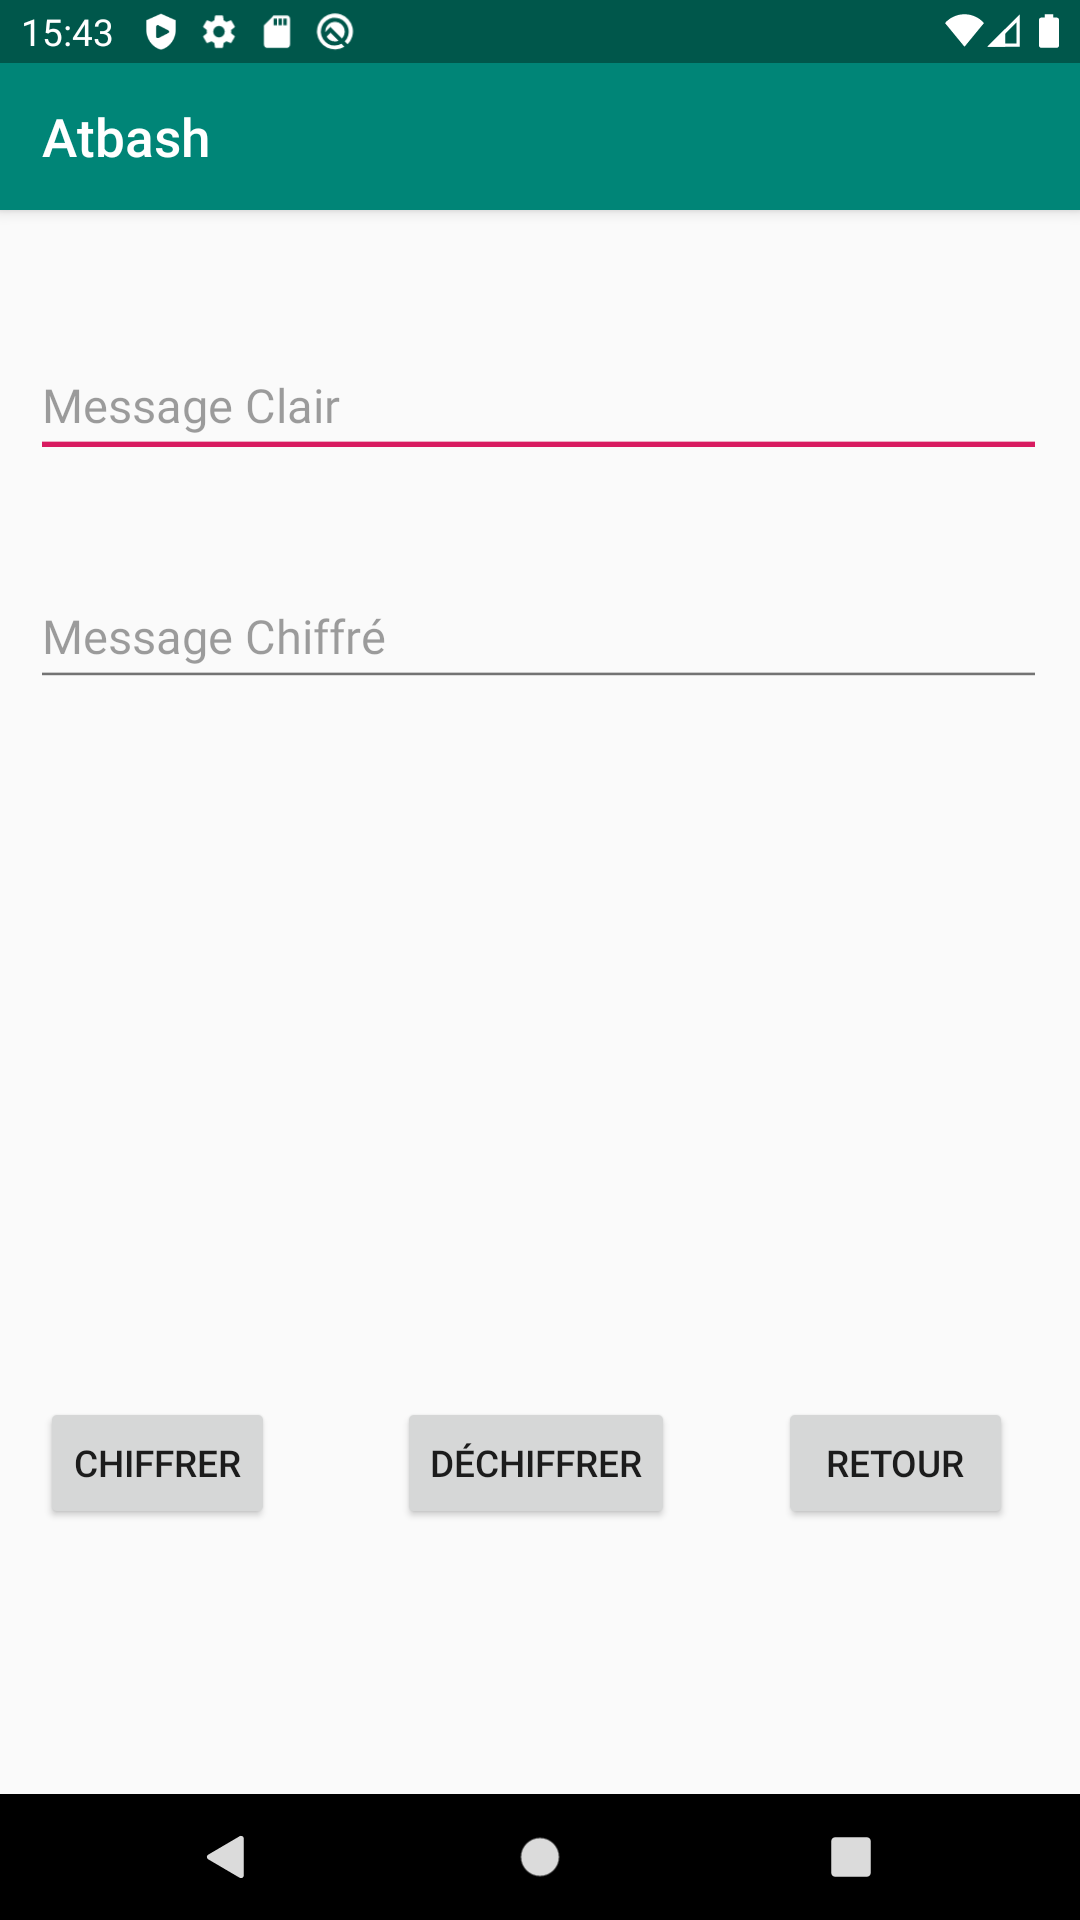
\includegraphics[width=.35\linewidth]{./img/atbash_ex.png} &
      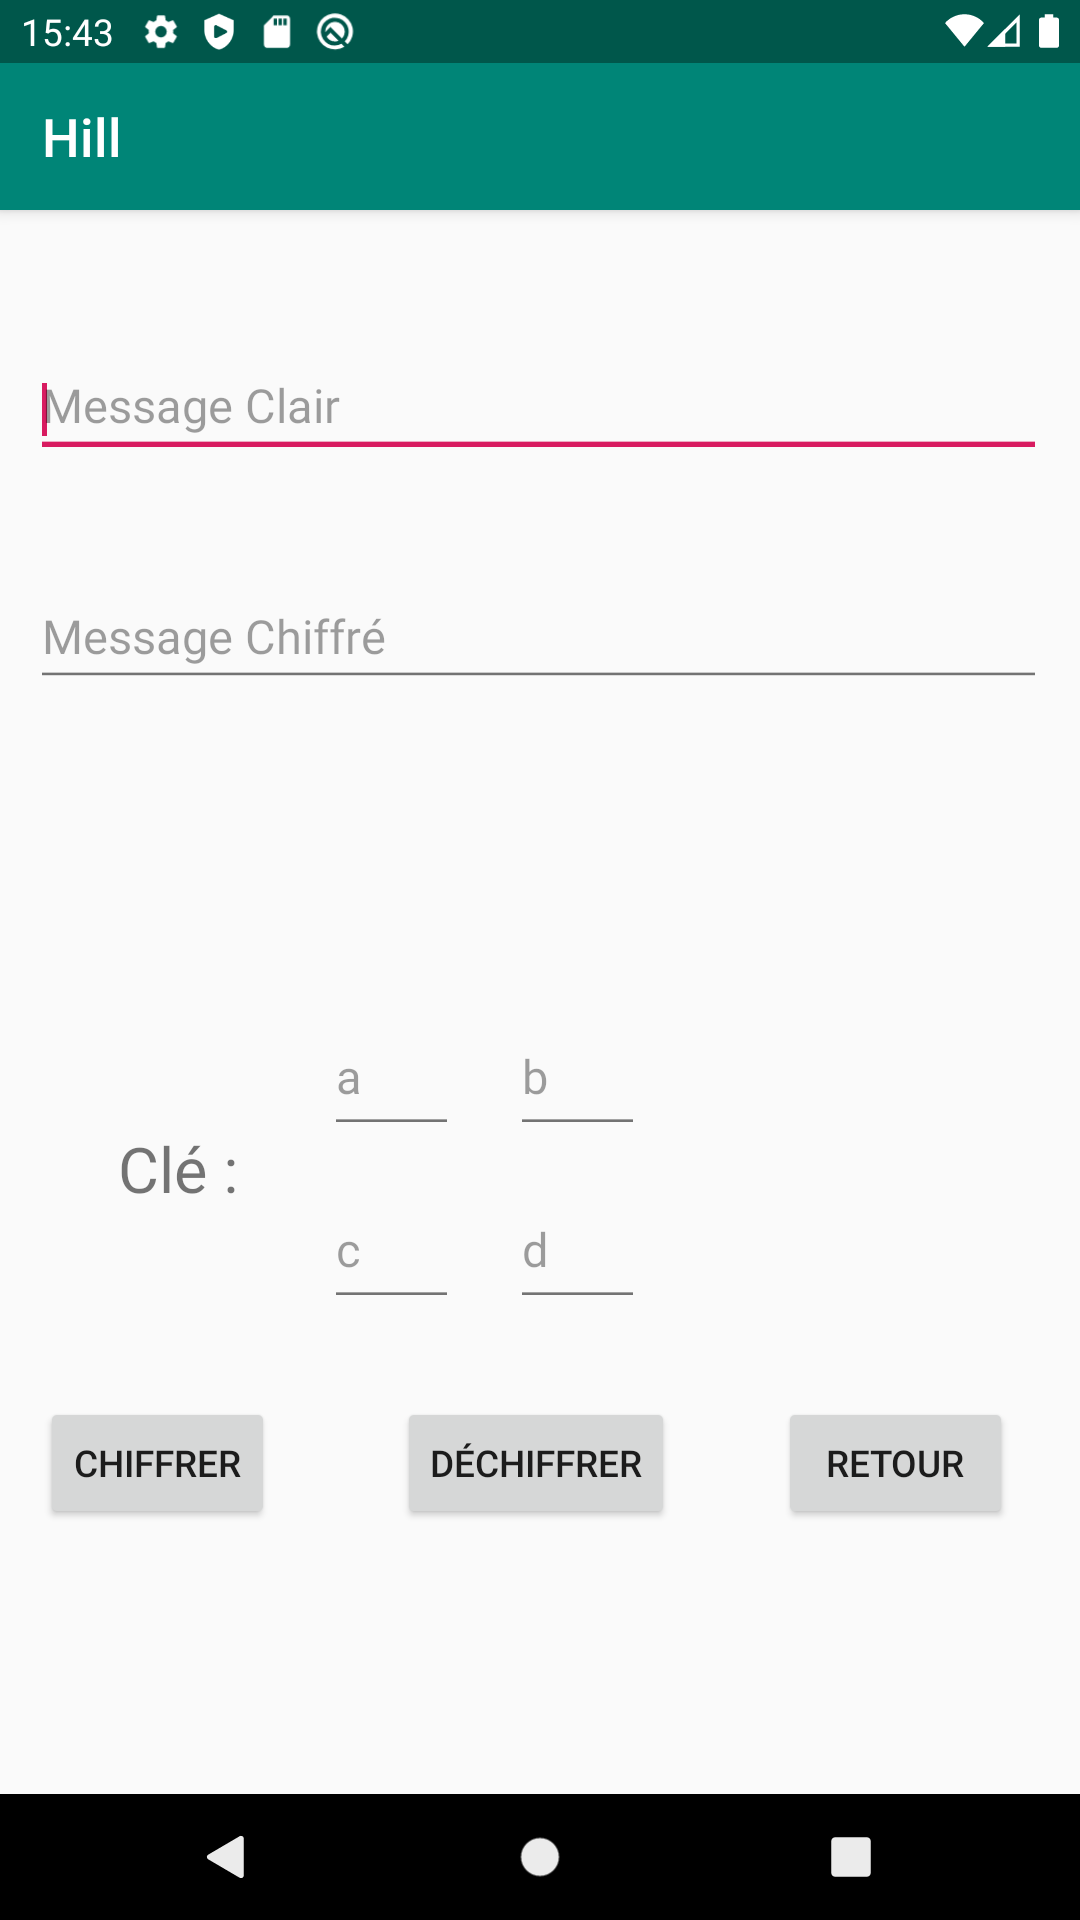
\includegraphics[width=.35\linewidth]{./img/hill_ex.png} \\
      Vue en sélectionnant Atbash & Vue en sélectionnant Hill\\
    \end{tabular}
    \caption{Différentes vues relatives à l'activité \textbf{CryptoDefaultActivity}\label{fig:exemple}}
\end{figure}

\begin{figure}[h!]
\centering
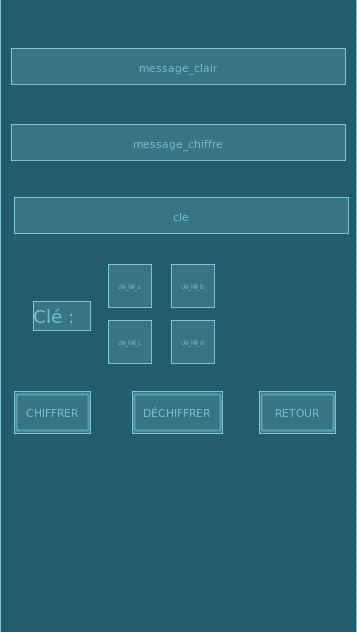
\includegraphics[scale=0.4]{./img/layout.png}
\caption{Structure de l'activité \textbf{CryptoDefaultActivity} avec le fichier \textit{crypto\_default\_layout.xml} \label{fig:layout}}
\end{figure}

\section{Algorithme de chiffrement/déchiffrement}

Tous les algorithmes que nous allons mentionner sont présents dans la classe \textbf{Crypto}. Elle contient toutes les méthodes publiques permettant de chiffrer/déchiffrer (pour chaque algorithme).
Chaque algorithme contient 3 paramètres :
\begin{itemize}
\item Message : Un \textbf{String} qui est le message à chiffrer ou déchiffrer.
\item La clé : Un \textbf{String} (ou un \textbf{int[]} pour Hill).
\item Un booléen \textbf{chiffre} qui va chiffrer s'il est vrai et déchiffrer sinon.
\end{itemize}
Elles renvoient toutes un \textbf{String} qui est le message chiffré ou déchiffré.

\subsection{Table ASCII étendue}

Nous travaillons pour la plupart des algorithmes de chiffrement avec la \textbf{table ASCII étendue}. En effet, elle est un prolongement de la table ASCII de base comprenant les codes de 0 à 127, en rajoutant 128 nouveaux caractères. Nous disposons des codes allant de 0 à 255 \textbf{(voir \ref{fig:cp437})}.

Cependant plusieurs encodages de cette table existent, nous utiliserons la norme \textbf{CP437}.
C'est la classe \textbf{ExtendedASCII.java} qui représente la table ASCII étendue. Elle contient plusieurs méthodes :
\begin{itemize}
\item \textbf{char getChar(int)} qui renvoie le caractère correspondant au code de la table ASCII étendue.
\item \textbf{int getASCIICode(char)} qui renvoie le code correspondant au caractère de la table ASCII étendue.
\item \textbf{int[] StringToAsciiCodeTable(String)} qui va transformer une chaîne de caractère en tableau d'entiers. Chaque entier étant le code ASCII correspondant. 
\item \textbf{String \textbf{AsciiCodeTableToString} (int[])} qui fait l'inverse de la méthode précédente. 

\end{itemize}
\vspace{1\baselineskip}

Pour la plupart des algorithmes de chiffrement nous allons utiliser principalement ces deux dernières méthodes. En effet, le but sera de transformer le message en tableau d'entiers contenant les différents codes ASCII étendue avec \textbf{StringToAsciiCodeTable}. Puis, de travailler dessus pour enfin restituer la chaîne représentant le message chiffré ou déchiffré avec \textbf{AsciiCodeTableToString}.
Ces deux méthodes gèrent également les caractères non affichables. La table contient plusieurs caractères de contrôle soit les codes ASCII de 0 à 31, le code 127 et le code 255. Ils seront représentés dans la chaîne par leur écriture en hexadécimal.
Exemple :
\begin{itemize}
\item \textbf{AsciiCodeTableToString(new int[]\{0 , 61 , 62 , 255\})} renvoie la chaîne \textbf{\textbackslash x00ab\textbackslash xff}.
\item \textbf{StringToAsciiCodeTable("Cc\textbackslash x7f")} renvoie le tableau \textbf{[43,63,127].}

\end{itemize}


\begin{figure}[h!]
\centering
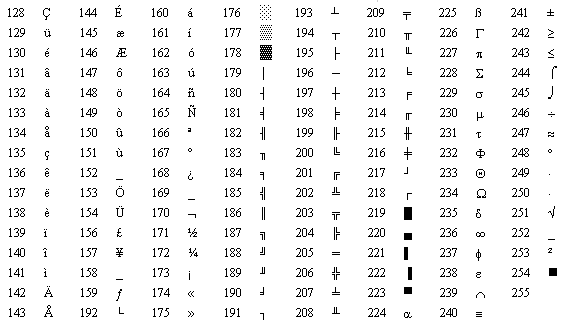
\includegraphics[scale=0.5]{./img/cp437.png}
\caption{128 nouveaux caractères de la table ASCII étendue avec la norme CP437 \label{fig:cp437}}
\end{figure}
\vspace{1\baselineskip}

\textbf{Nous pouvons maintenant parler de chaque algorithme de chiffrement}.

\subsection{Atbash}

Le chiffrage Atbash est un algorithme où l'on va substituer une lettre par son inverse dans la table ASCII étendue. Par exemple le caractère \textit{\textbf{"2"}} avec pour rang 50 dans la table devient le caractère ayant pour rang 200 (250-50). En général cela consiste en un décalage de $250 - i$. 
Le chiffrage et déchiffrage est totalement le même et est géré par la méthode \textbf{String atbash(String message)} de la classe Crypto.
\subsubsection{Exemple}
\begin{itemize}
\item On chiffre la chaine "\textbf{Heavy Metal}" représenté par les codes \textbf{[72,101,97,118,121,32,77,101,116,97,108]} deviennent \textbf{[183,154,158,137,134,223,178,154,139,158,147]} qui correspond à la chaîne "". \textbf{(voir figure \ref{fig:atbash})}
\item On déchiffre la chaîne obtenu et on ré-obtient \textbf{"Heavy Metal"}. \textbf{voir figure \ref{fig:cesar})} 
\end{itemize}

\subsection{César}\label{cesar}

Le chiffrage de César consiste à substituer un caractère par un autre. On décale chaque caractère du message $M$ par un certain nombre \textbf{$d$} pour obtenir le message chiffré $C$. On utilise la méthode \verb+String vigenere(String,String,boolean)+ de la classe \textbf{Crypto}.
Si on chiffre, le nouveau caractère \textbf{$C_{i}$} sera :

\[C_{i} = (M_{i}+d) \bmod 256 \]


Si on déchiffre, le nouveau caractère $C_{i}$ sera :

\[C_{i} = (M_{i}-d) \bmod 256 \]


\subsubsection{Exemple}
\begin{itemize}
\item Si on chiffre la chaîne "\textbf{Blink}" représenté par les codes \textbf{[66,108,105,110,107]} avec un décalage de \textbf{182} on obtient \textbf{[248,34,31,36,33]} qui donne la chaîne "\textbf{"\textbackslash x1f \$ !} (le code 31 représentant un caractère non affichable). \textbf{(Voir figure \ref{fig:cesar})}
\item Si on déchiffre cette chaîne avec le même décalage on ré-obtient \textbf{"Blink"}. \textbf{(Voir figure \ref{fig:cesar})}
\end{itemize}

\subsection{Vigenère}

Le chiffrement de Vigenère marche comme celui de César. \textbf{(voir \ref{cesar})} À la différence que pour chaque caractère $M_{i}$ du message $M$ on décalera du numéro du $i_{eme}$ caractère (modulo la longueur de la clé) de la clé $c$.
Donc pour $d = c_{i \bmod longueur(c)}$ si on chiffre ou déchiffre le nouveau caractère $C_{i}$ utilise la même formule que celle de César vu précédemment.
\subsubsection{Exemple}
\begin{itemize}
\item Si on prend le message \textbf{"Iron"} représentée par les codes \textbf{[73,114,111,110]}  avec la clé \textbf{"Maiden"} représentée par les codes \textbf{[77,97,105,100,101,110}. Le premier caractère est décalé de 77, le deuxième de 97 etc ... Ce qui donne les codes \textbf{[150,211,216,210]} ce qui donne la chaîne "". \textbf{(voir figure \ref{fig:vigenere})}
\item Si on reprend cette chaîne mais en déchiffrant on ré-obtient le message d'origine. \textbf{(voir figure \ref{fig:vigenere})}
\end{itemize}

\subsection{Chiffre de Playfair}

Le chiffrement de Playfair consiste en l'utilisation d'un carré de Polybe que l'on va renverser pour construire un \textbf{chiffre de Playfair}. Grace à celui ci on va substituer chaque couple de lettres avec un autre couple de lettres.
On utilise comme dit précédemment un \textbf{carré de Polybe} à la différence qu'ici, c'est un tableau de 6x6 cases contenant les lettres de l'alphabet et les chiffres. 

On utilise la fonction interne à la classe \textbf{Crypto} \verb+char[][] cleToPolybe(String cle)+ qui transforme une clé en un carré de polybe et \verb+char[][] polybeToPlayfair(char[][] polybe) + qui va prendre le carré de polybe et  réarranger celui-ci en lisant chaque colonne pour construire chaque ligne du chiffre de Playfair.

Pour le chiffrage et le déchiffrage l'algorithme marche exactement pareil pour chaque couple de lettres :
\begin{itemize}
\item \textbf{si les deux lettres sont sur des lignes et des colonnes différentes}, alors chaque lettre est remplacée par la lettre située sur la même ligne qu'elle mais sur la colonne de l'autre ligne.
\item \textbf{si les deux lettres sont sur la même ligne}, alors on remplace chaque lettre par la lettre immédiatement à sa droite (éventuellement, on revient à la première lettre de la ligne)
\item \textbf{si les deux lettres sont sur la même colonne}, alors on remplace chaque lettre par la lettre immédiatement sous elle (éventuellement, on revient à la première lettre de la colonne).
\item \textbf{si les deux lettres sont identiques} on insère entre les deux lettres une lettre rare (par exemple Q). On le fait en Java en utilisant un objet \textbf{StringBuffer} et la méthode \verb+insert(int offset , char c)+ qui permet d’insérer un caractère à un certain indice de la chaîne.
\end{itemize}

On réinsère ensuite les caractères spéciaux comme les espaces,la ponctuation etc en utilisant également un \textbf{String Buffer}. 

\subsubsection{Exemple}


\begin{itemize}
\item On chiffre la chaîne "\textbf{Dream Theater}" avec la clé "\textbf{Metropolis}". On transforme cette chaîne en mettant toutes les lettres en majuscules et en retirant tous les caractères ne correspondant pas à des chiffres ou des lettres (DREAMTHEATER). On obtient ce \textbf{chiffre de playfair} avec la clé :
\begin{center}
\begin{tabular}{|c|c|c|c|c|c|}
\hline
M & L & D & N & Y & 4 \\
\hline
E & I & F & Q & Z & 5 \\
\hline
T & S & G & U & 0 & 6 \\
\hline
R & A & H & V & 1 & 7 \\
\hline
O & B & J & W & 2 & 8 \\
\hline
P & C & K & X & 3 & 9 \\
\hline
\end{tabular} 
\end{center}
\vspace{1\baselineskip}

En faisant la substitution de chaque couple de lettres avec ce tableau et en respectant les 4 règles vu précédemment, \textbf{DR} devient \textbf{MH}, \textbf{EA} devient \textbf{IR} etc ... On obtient alors la chaîne \textbf{MHIRE RRFRSTO} en rajoutant l'espace présent dans la chaîne d'origine. \textbf{(voir figure  \ref{fig:playfair})}

\item On reprend ce message en utilisant la même clé et on ré-obtient le message "\textbf{DREAM THEATER}". \textbf{(voir figure  \ref{fig:playfair})}
 
\end{itemize}

\subsection{Chiffrage de Hill}\label{sub:Hill}

Le chiffrement de Hill consiste en une substitution par groupe de lettres (ici nous utiliserons pour des groupes de deux lettres). Chaque groupe de lettres $X_{i}$ du message $X$, sera codé par un vecteur $\begin{pmatrix}
x1\\
x2\\
\end{pmatrix}$ par rapport au rang de chaque lettre dans la table ASCII étendue. Pour obtenir le bloc $Y_{i}$ du message chiffré on va multiplier chaque vecteur $X_{i}$ par une matrice $M$ qui est la clé de forme :
$\begin{pmatrix}
a&b\\
c&d\\
\end{pmatrix}$
. Celle ci est correcte uniquement si son determinant est premier avec 256. (On vérifie dans le code si le pgcd du determinant et de 256 est égal à 1 avec la fonction \verb+int pgcd(int m, int n)+ de la classe Crypto).
On a donc : 

\[ Y_{i} = \begin{pmatrix}
y1\\
y2\\
\end{pmatrix} = \begin{pmatrix}
x1\\
x2\\
\end{pmatrix} \begin{pmatrix}
a&b\\
c&d\\
\end{pmatrix}  \]
Notons que chaque chiffre du bloc est ramené modulo 256. On obtient alors chaque caractère de la table ASCII étendue correspondant.
On représente la matrice $M$ et les blocs $X_{i}$ et $Y_{i}$ par un \verb+int[][]+ et des \verb+int[]+ en Java. 

Pour déchiffrer le message on applique le même principe mais en utilisant cette fois la matrice inverse de $M$ : $M^{-1}$. Pour ce faire on multiplie l'inverse du déterminant de M dans l'arithmétique modulo 256 p pour une certaine matrice $M^{'}$ : 

\[ M^{-1} = [det(M)]^{-1} \begin{pmatrix}
d&-b\\
-c&a\\
\end{pmatrix} \]

Pour calculer l'inverse du déterminant on utilise la fonction interne \verb+int modInverse(int a , int m)+.

\subsubsection{Exemple}
\begin{itemize}
\item On chiffre la chaîne "\textbf{Pantera}" avec la clé $\begin{pmatrix}
1&9\\
8&1\\
\end{pmatrix}$. On rajoute un caractère \textbf{"*"} pour que la longueur de la chaîne soit paire.
On obtient 4 groupes de deux lettres avec leur code de la table ASCII étendue associé :

\( X_1 = \begin{pmatrix}
80\\
97\\
\end{pmatrix} X_2 = 
\begin{pmatrix}
110\\
116\\
\end{pmatrix} X_3 = 
\begin{pmatrix}
101\\
114\\
\end{pmatrix} 
X_4 = \begin{pmatrix}
97\\
42\\
\end{pmatrix} \)
\vspace{1\baselineskip}

On obtient alors les blocs $Y_i$ : 

\( Y_1 = \begin{pmatrix}
185\\
225\\
\end{pmatrix} Y_2 = 
\begin{pmatrix}
130\\
228\\
\end{pmatrix} Y_3 = 
\begin{pmatrix}
103\\
154\\
\end{pmatrix} 
Y_4 = \begin{pmatrix}
219\\
50\\
\end{pmatrix} \)
\vspace{1\baselineskip}


On obtient alors le message \textbf{(voir figure \ref{fig:hill})} quand on regarde les caractères correspondants aux codes dans la table ASCII étendue. \textbf{(voir figure \ref{fig:hill})}
\vspace{1\baselineskip}

\item Si on déchiffre cette chaîne on ré-obtient le message "\textbf{Pantera*}" avec le caractère "*" qui avait été ajouté. \textbf{(voir figure \ref{fig:hill})}

\end{itemize} 
\subsection{Transposition Rectangulaire}\label{sub:transpo}

La transposition rectangulaire est un algorithme de transposition. C'est à dire que l'on va changer l'ordre des caractères de la chaîne. Le but est d'utiliser un tableau qui contiendra tous les caractères du message.

(Dans notre cas pour préserver les caractères non affichables on utilise un tableau d'entier \verb+int[][]+ en Java). 


 Pour commencer soit $n$ la longueur de la clé chaque ligne du tableau aura $n$ éléments. Ensuite on créé une ligne $R$ qui contiendra le "rang" de chaque caractère du tableau. Celui ayant son code le plus petit dans la table ASCII étendue  aura comme "rang" \textbf{1}, puis le deuxième plus petit \textbf{2} etc ... (Dans notre code en Java elle n'est pas directement incluse dans le tableau vu précédemment mais stockée dans un \verb+int[]+ à part).
\begin{itemize}
\item \textbf{Si on chiffre} on va remplir le tableau ligne par ligne avec le message d'origine. Pour obtenir le message chiffré on va le construire en lisant la colonne correspondant à l'indice de l’élément de $R$ numéroté 1, puis la colonne avec l'indice numéroté 2, etc ...  
\item \textbf{Si on déchiffre} on doit reconstituer le tableau pour savoir quelle taille font les différentes colonnes. Soit $n$ la longueur de la clé, et $m$ la longueur du message. 
\begin{itemize}
\item Si $n$ est un multiple de $m$ alors toutes les colonnes font une taille de $m/n$.
\item Sinon pour $m/n$ on a $q$ le quotient et $r$ le reste. On aura alors les $r$ premières colonnes qui ont une taille de $q+1$ et les $n-r$ autres qui ont une taille de $q$.
\end{itemize}
On remplit alors le tableau avec chaque caractère du message par colonne. D'abord la colonne correspondant à l'indice de l'élément de $R$ numéroté 1 puis 2 etc ...
On lit ensuite le tableau ligne par ligne pour obtenir le message déchiffré.
\end{itemize}

La création de la ligne $R$ se fait avec la fonction interne \verb+int[] cleToNumeroAssocie(String cle)+.

\subsubsection{Exemple}
(Les cases vides seront notées avec le caractère $\emptyset$).
\begin{itemize}
\item On chiffre la chaîne $M$ "\textbf{Ich tu der weh}" avec la clé $N$ "\textbf{Rammstein}". On regardant chaque code ASCII étendue des caractères de la clé. On obtient alors ce tableau $R$ : 
\vspace{1\baselineskip}

\begin{center}
\begin{tabular}{|c|c|c|c|c|c|c|c|c|}
\hline
R & a & m & m & s & t & e & i & n\\
\hline
1 & 2 & 5 & 6 & 8 & 9 & 3 & 4 & 7\\
\hline
\end{tabular}
\end{center}
\vspace{1\baselineskip}

On obtient alors le tableau pour chiffrer en remplissant avec le message $m$ : 
\vspace{1\baselineskip}

\begin{center}
\begin{tabular}{|c|c|c|c|c|c|c|c|c|}
\hline
R & a & m & m & s & t & e & i & n\\
\hline
1 & 2 & 5 & 6 & 8 & 9 & 3 & 4 & 7\\
\hline
I & c & h &  & t & u &  & d & e\\
\hline
r &  & w & e & h & $\emptyset$ & $\emptyset$ & $\emptyset$ & $\emptyset$\\
\hline
\end{tabular}
\end{center}
\vspace{1\baselineskip}

En lisant la colonne 1 puis 2 etc ... On obtient la chaîne chiffrée $C$ "\textbf{Irc  dhw eethu}" (il y a deux caractères " " entre le c et le d). \textbf{(Voir figure \ref{fig:transpo})}
\vspace{1\baselineskip}


\item \textbf{On déchiffre} la chaîne $C$ "\textbf{Irc  dhw eethu}". On garde le même tableau $R$.

On a la longueur du mot $C$ : $m=14$ et la longueur de la clé $N$ : $n = 9$. 

Pour $m/n$ on a alors $q=1$ et $r = 5$. Les 5 premières colonnes ont une taille de 2 ($q+1$) et les 4 autres une taille de 1 ($q$). On remplit la colonne numérotée 1 avec "Ir" puis celle numérotée 2 avec "c " etc ...  On ré-obtient alors le tableau de chiffrage initial :
\vspace{1\baselineskip}

\begin{center}
\begin{tabular}{|c|c|c|c|c|c|c|c|c|}
\hline
R & a & m & m & s & t & e & i & n\\
\hline
1 & 2 & 5 & 6 & 8 & 9 & 3 & 4 & 7\\
\hline
I & c & h &  & t & u &  & d & e\\
\hline
r &  & w & e & h & $\emptyset$ & $\emptyset$ & $\emptyset$ & $\emptyset$\\
\hline
\end{tabular}
\end{center}
\vspace{1\baselineskip}

On lit ensuite le tableau ligne par ligne pour ré-obtenir le message $M$ : "\textbf{Ich tu der weh}". \textbf{(Voir figure \ref{fig:transpo})}



\end{itemize}

\subsection{DES}

Le \textbf{DES} (Data Encryption Standard) est un algorithme de sur-chiffrement, c'est à dire que l'on va chiffrer ou déchiffrer avec des clés différentes à chaque fois. Il prend en entrée un bloc de 64 bits et une clé de 64 bits. Si le message fait moins de 64 bits (8 caractères sur 8 bits) on le complète avec des zero. Si il fait plus on sépare le message en blocs de 64bits et on appliquera l'algorithme pour chacun de ces blocs. 

C'est la fonction \verb+String[] messageToBlocs(int[] message)+ qui transforme le tableau de code ASCII étendue de notre message en blocs de 64 bits. (Nos chaînes de bits sont représentées via des \verb+String+ en Java). 

L'algorithme se déroule alors comme suit : 

\begin{itemize}
\item \textbf{Diversification des clés : } À partir de la clé donnée en entrée on dérive 16 sous-clés de 48 bits. C'est la fonction \verb+String[] diversificatonCle(String cle)+ qui crée un tableau contenant les 16 clés $K_i$.
\item \textbf{Permutation initiale : } Pour chaque blocs de 64 bits on applique une permutation initiale (on va changer chaque bits de place). C'est la fonction \verb+String permutationInitiale(String bloc)+ qui s'applique. On obtient alors un bloc de 64 bits que l'on va séparer en deux blocs de 32 bits $G_0$ et $D_0$.
\item \textbf{Schéma de Feistel : } On va calculer avec 16 itérations (de 1 à 16) tous les $G_i$ et $D_i$ en suivant ce schéma tel que : 
\begin{itemize}
\item \(G_{i-1} = D_{i-1}\)
\item \(D_{i-1} = G_{i-1} \bigoplus f_{confusion}(D_{i-1} , K_i)\)
\end{itemize}
Les blocs $D_i$ et $G_i$ étant stockés dans deux tableaux de \verb+String[]+ . Pour l'opérateur $\bigoplus$ on utilise une fonction interne \verb+String XOR (String blocA,String blocB)+ qui renvoie le résultat de $A \bigoplus B$. Enfin la fonction de confusion renvoie un bloc de 32 bits prenant en entrée un bloc de 32 bits et une clé diversifiée $K_i$ de 48 bits, c'est la fonction \verb+String fonctionConfusion(String bloc32 , String cleDiversifie)+ qui calcule ce bloc.

\item \textbf{Permutation finale : } On applique enfin à G16 D16 une permutation finale et on obtient alors le message chiffré. On le fait avec la fonction interne \verb+String permutationFinale(String bloc)+. 
\end{itemize}
\vspace{1\baselineskip}


Pour déchiffrer on va appliquer le même principe mais en utilisant les clés $K_i$ dans l'ordre inverse à chaque itération (d'abord $K_{16}$ puis $K_{15}$ etc ...).
\vspace{1\baselineskip}

\textit{(L'algorithme dispose également d'une option pour chiffrer/déchiffrer uniquement avec un nombre hexadécimal en activant une checkbox).}

\subsubsection{Exemple}

\textbf{Pour des messages avec des caractères de la table ASCII étendue : }
\begin{itemize}

\item \textbf{On chiffre} le message "\textbf{Gojira}" avec la clé "\textbf{\textbackslash x0123456789abcdef}". Il fait 6 caractères donc 48bits on le complète alors avec des 0 et on obtient le bloc en binaire : 
\[ M = 0100\ 0111\ 0110\ 1111\ 0110\ 1010\ 0110\ 1001\ 0111\ 0010\ 0110\ 0001\ 0000\ 0000\ 0000\ 0000 \]
Après passage dans l'algorithme on obtient le bloc chiffré : 
\[ C = 0101\ 0101\ 0000\ 1010\ 0101\ 0100\ 0111\ 0011\ 0100\ 0011\ 0100\ 0000\ 1101\ 1101\ 0100\ 0001 \]
Ce qui pour chaque octet représente les caractères de la table ascii étendue numéro \textbf{[85,10,84,115,67,64,221,65]} (un caractère étant codé sur 8 bits). \textbf{(voir figure \ref{fig:des})}
\vspace{1\baselineskip} 

\item \textbf{On déchiffre} la chaîne $C$ avec la même clé. On ré-obtient alors le bloc $M$ et le message "\textbf{Gojira}". \textbf{(voir figure \ref{fig:des})}

\end{itemize}
\textbf{Pour des messages en hexadécimal : }
\begin{itemize}
\item \textbf{On chiffre} le message en hexadécimal "\textbf{\textbackslash x23456789abcdef01}" avec la clé "\textbf{\textbackslash x0123456789abcdef}". On a alors le bloc à chiffrer : 
\[ M = 0010\ 0011\ 0100\ 0101\ 0110\ 0111\ 1000\ 1001\ 1010\ 1011\ 1100\ 1101\ 1110\ 1111\ 0000\ 0001\]
Après passage dans l'algorithme on obtient le bloc : 
\[C = 1010\ 0100\ 0111\ 0110\ 0000\ 0110\ 1010\ 1111\ 0001\ 0011\ 0010\ 1110\ 1110\ 1111\ 1111\ 0111\]
Ce qui correspond à "\textbf{\textbackslash xa47606af132eeff7}" en hexadécimal. \textbf{(voir figure \ref{fig:des_hex})}
\vspace{1\baselineskip} 

\item Si on déchiffre $C$ on ré-obtient le bloc $M$ soit "\textbf{\textbackslash x23456789abcdef01}". \textbf{(voir figure \ref{fig:des_hex})}
\end{itemize}

\subsection{Algorithme Surprise !}

Nous allons présenter ici l'élaboration d'un algorithme surprise. Celui-ci prend en entrée un message représenté par une chaîne de caractères $M$ dans la table ASCII étendue et une clé $C$ elle aussi une chaîne de caractères. Il est composé de deux étapes : 
\begin{itemize}
\item \textbf{Transposition du message $M$ : } On va effectuer une \textbf{Transposition Rectangulaire} de $M$ avec la clé $C$. 
\item \textbf{Substitution de $M$ : } On va substituer chaque caractère de $M$ par un caractère dans la \textbf{table des émojis}. 
\end{itemize}

\subsubsection{Table des émojis}

Chaque émoji est représenté par un code \textbf{Unicode}. En effet toute la table des émojis est en fait une extension de la table \textbf{Unicode}. 
Actuellement on est à la version 13 de celle-ci (30/01/2020) et on compte \textbf{1809} émojis pour les codes allant de \textbf{U+1F600} à \textbf{U+1F3F4}.

\begin{figure}[h!]
\centering
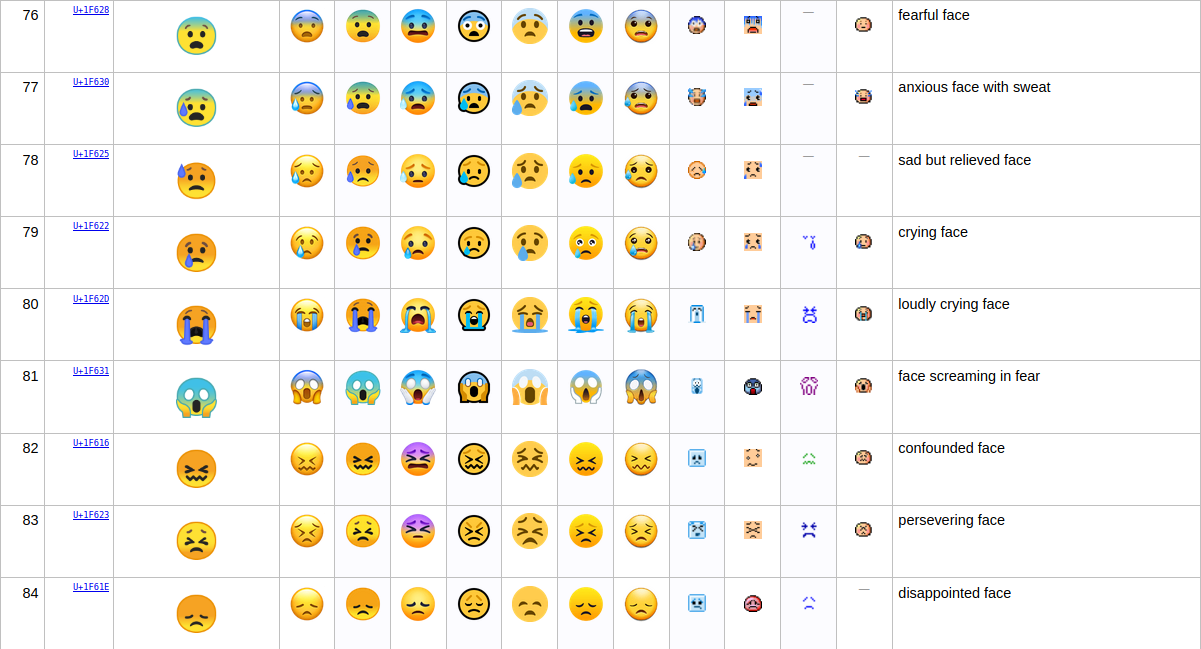
\includegraphics[scale=0.35]{./img/emoji.png}
\caption{Aperçu de la table de émojis \label{fig:emoji}}
\end{figure}


Ce nombre d'émojis augmente encore si on prend en compte les variantes de certains émojis (couleurs de peau etc ...) disposant de plusieurs \textbf{unicode}.

\subsubsection{Création de cette table en Java}

Bien évidemment le langage \textbf{Java} que nous utilisons dans Android Studio ne dispose pas de ces émojis en natif nous avons donc besoin d'un objet pour les représenter.

Nous utilisons deux librairies : 
\begin{itemize}
\item \textbf{emoji-java} de \textbf{vdurmont} (\href{https://github.com/vdurmont/emoji-java}{https://github.com/vdurmont/emoji-java}) : Qui via son objet \textbf{EmojiManager} permet d'obtenir un tableau d’émoji \verb+Emoji[]+. On peut ensuite récupérer \textbf{l'unicode} d'un émoji avec la méthode \verb+String getUnicode()+ de l'objet \textbf{Emoji} pour pouvoir l'afficher \textbf{(L'émulateur Android comprenant ces caractères Unicode)} .
\item \textbf{emoji4j} de \textbf{kcthota} (\href{https://github.com/kcthota/emoji4j}{https://github.com/kcthota/emoji4j}) : Qui nous permet de "parser" une chaîne d'Emoji pour récupérer les caractères \textbf{hexadécimaux HTML} de chaque émoji avec \verb+EmojiUtils.hexHtmlify(String s)+. (Java ne sachant pas lire des émojis encore une fois).
\end{itemize}
\vspace{1\baselineskip} 


On créé pour cela une classe \textbf{EmojiTable} : 

\begin{verbatim}
public class EmojiTable {

Emoji[] emojitable =  EmojiManager.getAll().toArray(new Emoji[EmojiManager.getAll().size()]);
Emoji[] emojitable_simplified = new Emoji[848];


    public EmojiTable(){

        //Emoji simplifié de [0,143] [146,627] [638,836] [1048,1073]
        int compteur=0;
        for (int i=0 ; i<emojitable.length; i++){

            if( (i>=0 && i<=143) || (i>=146 && i<=627) || (i>=641 && i<=836) || (i>=1048 && i<=1073)){

                emojitable_simplified[compteur] = emojitable[i];
                compteur++;
            }
        }
    }
    public Emoji[] getEmojitable_simplified(){return  this.emojitable_simplified;}

	// récupère le numéro d'un emoji dans la table en fonction de son code hexHTML
    public int getEmojiNumber(String emoji_html_hexa){


        for (int i=0 ; i<tab.length ; i++){

            if(emoji_html_hexa.equals(this.emojitable_simplified[i].getHtmlHexadecimal())) return i;}

        return -1;
}
\end{verbatim}

Nous travaillons sur une \textbf{table d'émoji simplifiée}. En effet comme dit précédemment certains émojis disposent de plusieurs codes Unicode (par exemple les émojis disposant de plusieurs couleurs de peau) donc, de plusieurs nombres Hexadécimaux HTML. Cela rend compliqué le "parse" avec la méthode \verb+EmojiUtils.hexHtmlify(String s)+. Nous gardons donc uniquement les émojis composés d'un seul code \textbf{Unicode}, ce qui nous donnent quand même 848 émojis affichables.

\textit{\textbf{(De plus la table des émojis de la librairie  emoji-java n'est pas à jour avec la table actuelle ... })}
\subsubsection{Fonctionnement de l'algorithme}

Après avoir effectué une \textbf{transposition rectangulaire} sur le message d'origine on va décaler chaque caractère d'un certain nombre. On a $M$ le message transposé, $Ci$ chaque code ASCII étendue de la clé, $R$ le tableau des numéros associé à la clé (le même que pour la transposition rectangulaire voir \ref{sub:transpo}) et pour chaque code  $M_i$ on décale tel que :  

\[ M'_i = (M'_i + (\   (|C| \times R_{i \bmod |C|}) \times C_{i \bmod |C|})) \bmod 848 \]

Pour chaque caractère $C_i$ du message chiffré on prend dans la table des émojis (\verb+Emoji[]+) l'unicode de l'émoji numéro $M'_i$ avec la méthode de l'objet Emoji \verb+getUnicode()+. On obtient ainsi un message uniquement composé d'émojis. (Android sachant afficher un émoji en connaissant l'unicode associé)
\vspace{1\baselineskip} 

\textbf{Pour le déchiffrage} on effectue l'opération inverse on décale dans l'autre sens modulo 848 puis on fait une transposition rectangulaire en déchiffrant.
Le soucis est que l'on a comme message à déchiffrer des émojis que \textbf{Java} ne sait pas reconnaître. On utilise alors l'objet \textbf{EmojiUtils} et la méthode \verb+hexHtmlify(String s)+ qui nous renvoie la représentation de chaque émoji en hexadécimal html (l'objet EmojiUtils ne disposant pas d'une méthode pour donner la représentation en Unicode). 

Par exemple l'émoji "pomme" a pour code \textbf{\&\#x1f34e}.

\subsubsection{Exemple}

\begin{itemize}
\item \textbf{On chiffre} le message "\textbf{Machine Head}" avec la clé "\textbf{Locust}". On transpose chaque caractère de la chaîne "\textbf{MecHa iandhe}" avec les codes ASCII \textbf{[77,101,99,72,97,32,105,97,110,100,104,101,]}.
Chaque code est décalé et ramené modulo 848 on obtient alors les émojis numéro \textbf{[533,403,439,44,313,120,561,399,450,72,320,189]} de notre table des émojis. \textbf{(voir figure \ref{fig:surprise})}

\item \textbf{On déchiffre} les émojis obtenus en récupérant pour chacun leur code html hexadécimal : \&\#x1f345; \&\#x1f4dd; \&\#x1f3ac; \&\#x1f61f; \&\#x1f390; \&\#x261d;

\&\#x1f5fd; \&\#x1f4ec; \&\#x1f47e; \&\#x1f478; \&\#x1f38b; \&\#x1f436;
\vspace{1\baselineskip} 

On peut alors récupérer chaque numéro d'émoji correspondant, en comparant leur code html hexadécimal avec \verb+Emoji+.\verb+getHtmlHexadecimal()+. 

On peut déchiffrer le message et on ré-obtient la chaine "\textbf{Machine Head}". \textbf{(voir figure \ref{fig:surprise})}

\end{itemize}


\subsection{RSA}

L'algorithme \textbf{RSA} est un chiffrement asymétrique, c'est à dire que l'on va utiliser une clé publique pour chiffrer et une clé privée pour déchiffrer.

La clé publique est un couple d'entiers naturels $(e,n)$ et la clé privée un couple d'entiers naturels $(d,n)$.

Notre algorithme prend en entrée deux nombres premiers $P$ et $Q$, un message $M$ qui est un entier et renvoie un nombre $C$ qui est le message chiffré. Il se déroule comme suit : 

\begin{itemize}
\item On choisit $P$ et $Q$ deux nombres premiers.
\item On calcule $n = P \times Q$ et $\phi(n) = (P-1)\times(Q-1)$.
\item On choisit un entier $e$ tel que $e$ est premier avec $\phi(n)$ (dans notre cas on prend $e > q$ tel que le pgcd de $e$ et $\phi(n)$ soit égal à 1).
\item On calcule $d$ qui est l'inverse de $e$ dans l'arithmétique modulo $\phi(n)$ (on utilise la fonction interne \verb+modInverse(int a , int m)+ utilisée dans le chiffrage de \textbf{Hill} voir \ref{sub:Hill}).
\item On a maintenant la clé publique $(e,n)$ et la clé privée $(d,n)$.
\end{itemize} 
\vspace{1\baselineskip}

Pour obtenir le message chiffré $C$ on a :
\(C \equiv M^e  \ \ \ \ (\bmod \ n\))

Pour déchiffrer et ré-obtenir le message $M$ on a :
\(M \equiv C^d  \ \ \ \	(\bmod \ n\))
\vspace{1\baselineskip}

Si le message $M$ ou $C$ est supérieur ou égal à $n$ alors, on les divise en blocs inférieurs strictement à $n$. On le fait avec la fonction interne \verb+String[] mToStringBlocs(int m, int n)+ qui va prendre un nombre m et n et qui va diviser le message m en blocs inférieurs strictement à $n$. 

Enfin pour le calcul de $M$ ou $C$ le soucis est que $M^e$ ou $C^d$ sont des très grand nombres. Java ne peut donc pas les stocker efficacement dans un type \verb+int+ et effectuer le modulo. On utilise alors l'objet \textbf{BigInteger} qui déjà stocke ces très grands nombres. Et notamment il dispose d'une méthode \verb+ BigInteger modPow(BigInteger exponent , BigInteger modulus)+ qui nous permettra de calculer $M$ et $C$.

\begin{verbatim}
//chiffrage ou déchiffrage des blocs
String[] blocsM = mToStringBloc(M , n);

//utilisation de BigInteger

BigInteger e_big =  BigInteger.valueOf((long) e);
BigInteger d_big = BigInteger.valueOf((long) d);
BigInteger n_big = BigInteger.valueOf((long) n);

for (int i=0 ; i<blocsM.length ; i++){

	BigInteger bloc_chiffre_dechiffre = BigInteger.valueOf(0);
    BigInteger bloc = BigInteger.valueOf(Long.parseLong(blocsM[i]));

    if(chiffre) bloc_chiffre_dechiffre = bloc.modPow(e_big,n_big);

    if(!chiffre) bloc_chiffre_dechiffre = bloc.modPow(d_big , n_big);

	resultat+=bloc_chiffre_dechiffre.toString();

   }

   return resultat;
\end{verbatim}


\subsubsection{Exemple}

On prend $P = 83$ et $Q=89$ : 
\begin{itemize}
\item On a $n = 7387$ et $\phi(n) = 7216$
\item On choisit $e = 91 $ et on calcule $ d \equiv 91^{-1} \ \ \ \ (\bmod \ 7987)$
\item On a la clé publique $(91 , 7387)$ et la clé privée $(5075 , 7387)$  
\end{itemize}
\vspace{1\baselineskip}

\begin{itemize}
\item \textbf{On chiffre} le message $M = 6882326$. $M \geq n$ donc on divise $M$ en deux blocs $M_1 = 6882$ et $M_2 = 326$ .

On alors $C_1 \equiv  6882 ^{91} \ \ \ (\bmod\ 7387) = 7301$ et $C_2 \equiv  326 ^{91} \ \ \ (\bmod\ 7387) = 1658$

Le message chiffré $C$ est \textbf{73011658} \textbf{(voir figure \ref{fig:RSA})}
\vspace{1\baselineskip}

\item \textbf{On déchiffre} le message $C = 73011658$. $C \geq n$ donc on divise $C$ en deux blocs $C_1 = 7301$ et $C_2 = 1658$ .

On alors $M_1 \equiv  7301 ^{5075} \ \ \ (\bmod\ 7387) = 6882$ et $M_2 \equiv  1658 ^{5075} \ \ \ (\bmod\ 7387) = 326$

Le message déchiffré $M$ est \textbf{6882326} \textbf{(voir figure \ref{fig:RSA})}
\end{itemize}

\section{Conclusion}

Nous avons présenté plusieurs algorithmes de chiffrement durant ce rapport. Chacun d'entre eux repose sur des techniques particulières de chiffrement, mais la plupart sont très peu résistant à des attaques de type "brute force" ou à des attaques statistiques même en utilisant plus de caractères (table ASCII étendue). Le \textbf{DES} quand à lui a été remplacé car il était sensible à des attaques sur les clés. Son vrai successeur est \textbf{l'AES} (Advanced Encryption Standard) car celui-ci n'utilisant pas de schéma de Feistel a une complexité plus faible que celle du DES. Il utilise moins de mémoire et est beaucoup plus résistant aux attaques (utilisant des longueurs de clés de 128, 192, 256 bits).

\textbf{L’algorithme RSA} est quand à lui très résistant aux attaques à condition d'utiliser des nombres premiers très grands pour la génération des clés(c'est pour cela qu'il est très utilisé dans l'échange de données confidentielles). En effet "casser" RSA nécessite d'utiliser une factorisation en produits de facteurs premiers, qui est un algorithme ayant une complexité \textbf{exponentielle}. Cependant l'algorithme de \textbf{Shor} un algorithme quantique est capable de le faire pour un entier $N$ en un temps $O((\log N)^3)$ ce qui pourrai complètement mettre à mal la sécurité de \textbf{RSA}, bien que l'on soit encore très loin d'avoir des ordinateurs quantiques le permettant.




\section{Annexe}

\begin{figure}[b!]
    \centering
    \begin{tabular}{cc}
      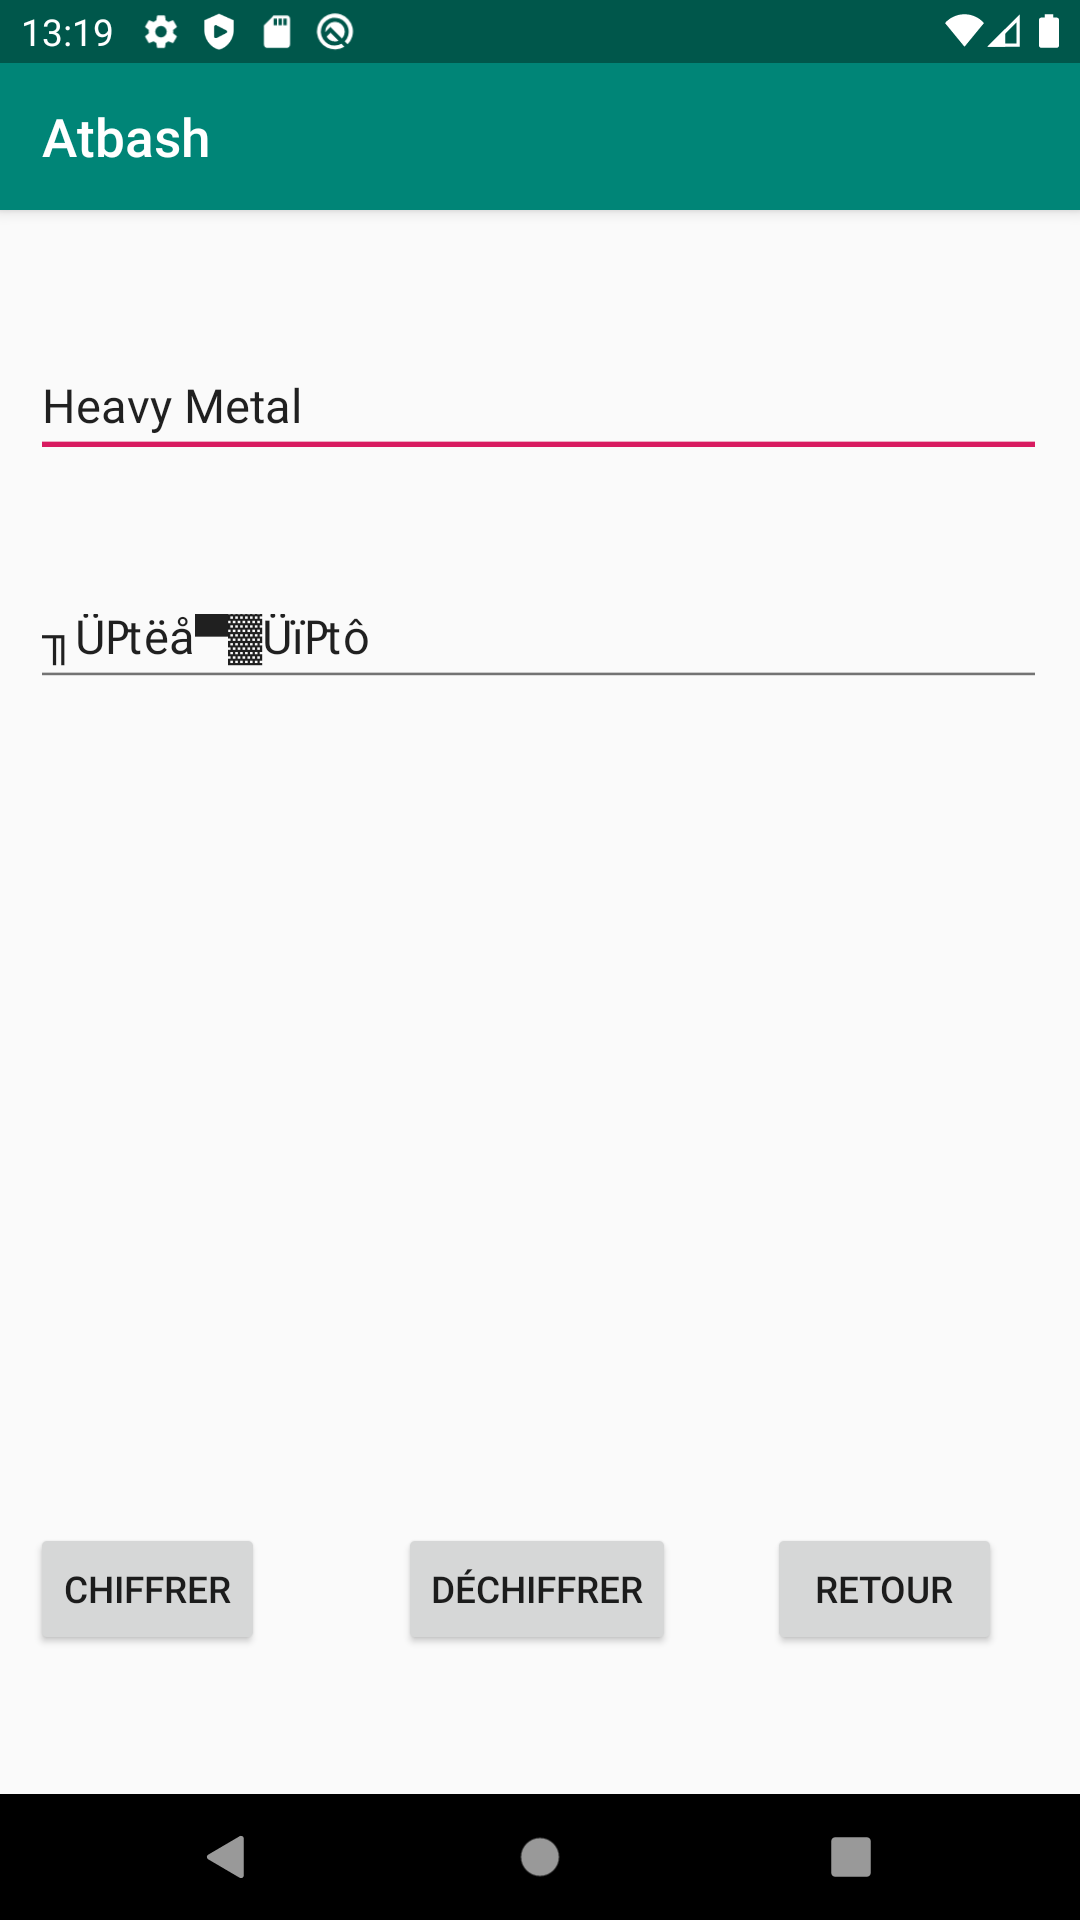
\includegraphics[width=.35\linewidth]{./img/atbash_e.png} &
      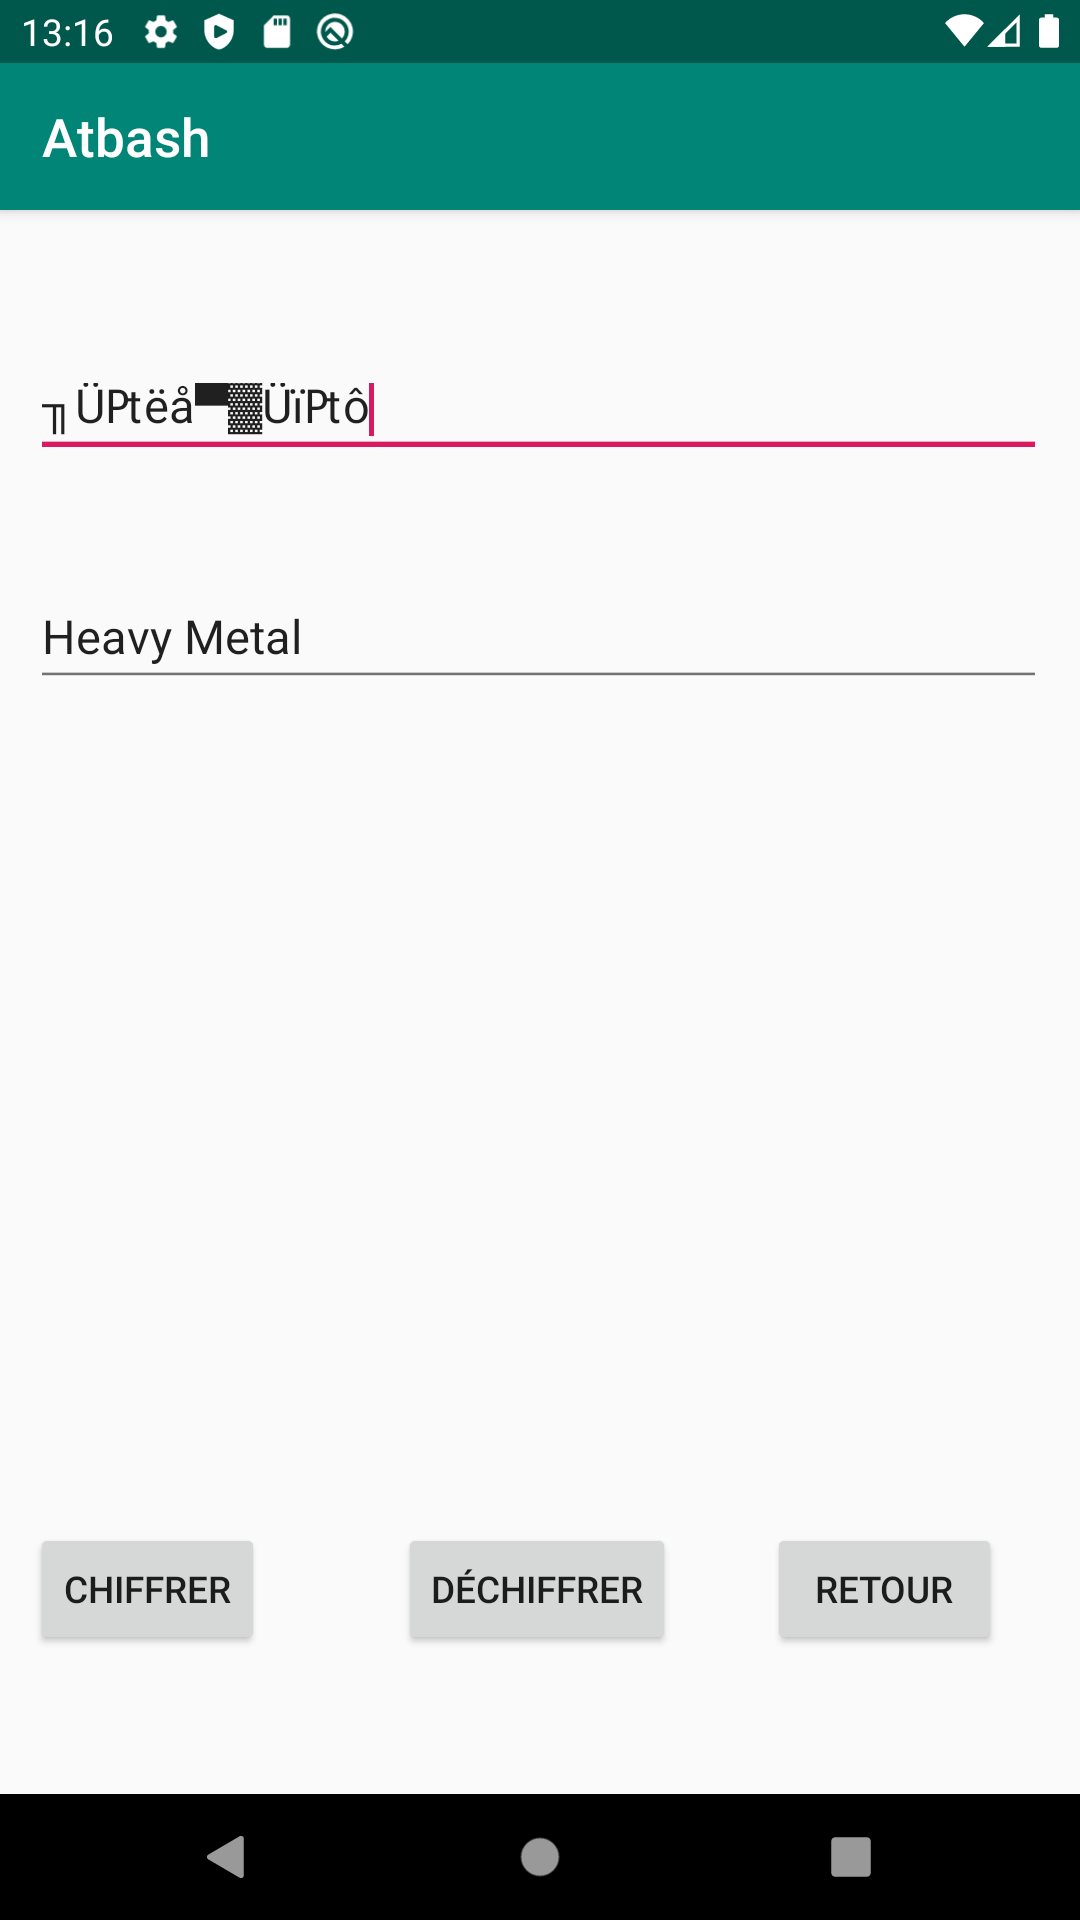
\includegraphics[width=.35\linewidth]{./img/atbash_d.png} \\
      Chiffrage de "Heavy Metal" & Déchiffrage de ""\\
    \end{tabular}
    \caption{Chiffrage et déchiffrage avec \textbf{Atbash}}\label{fig:atbash}
\end{figure}

\begin{figure}[b!]
    \centering
    \begin{tabular}{cc}
      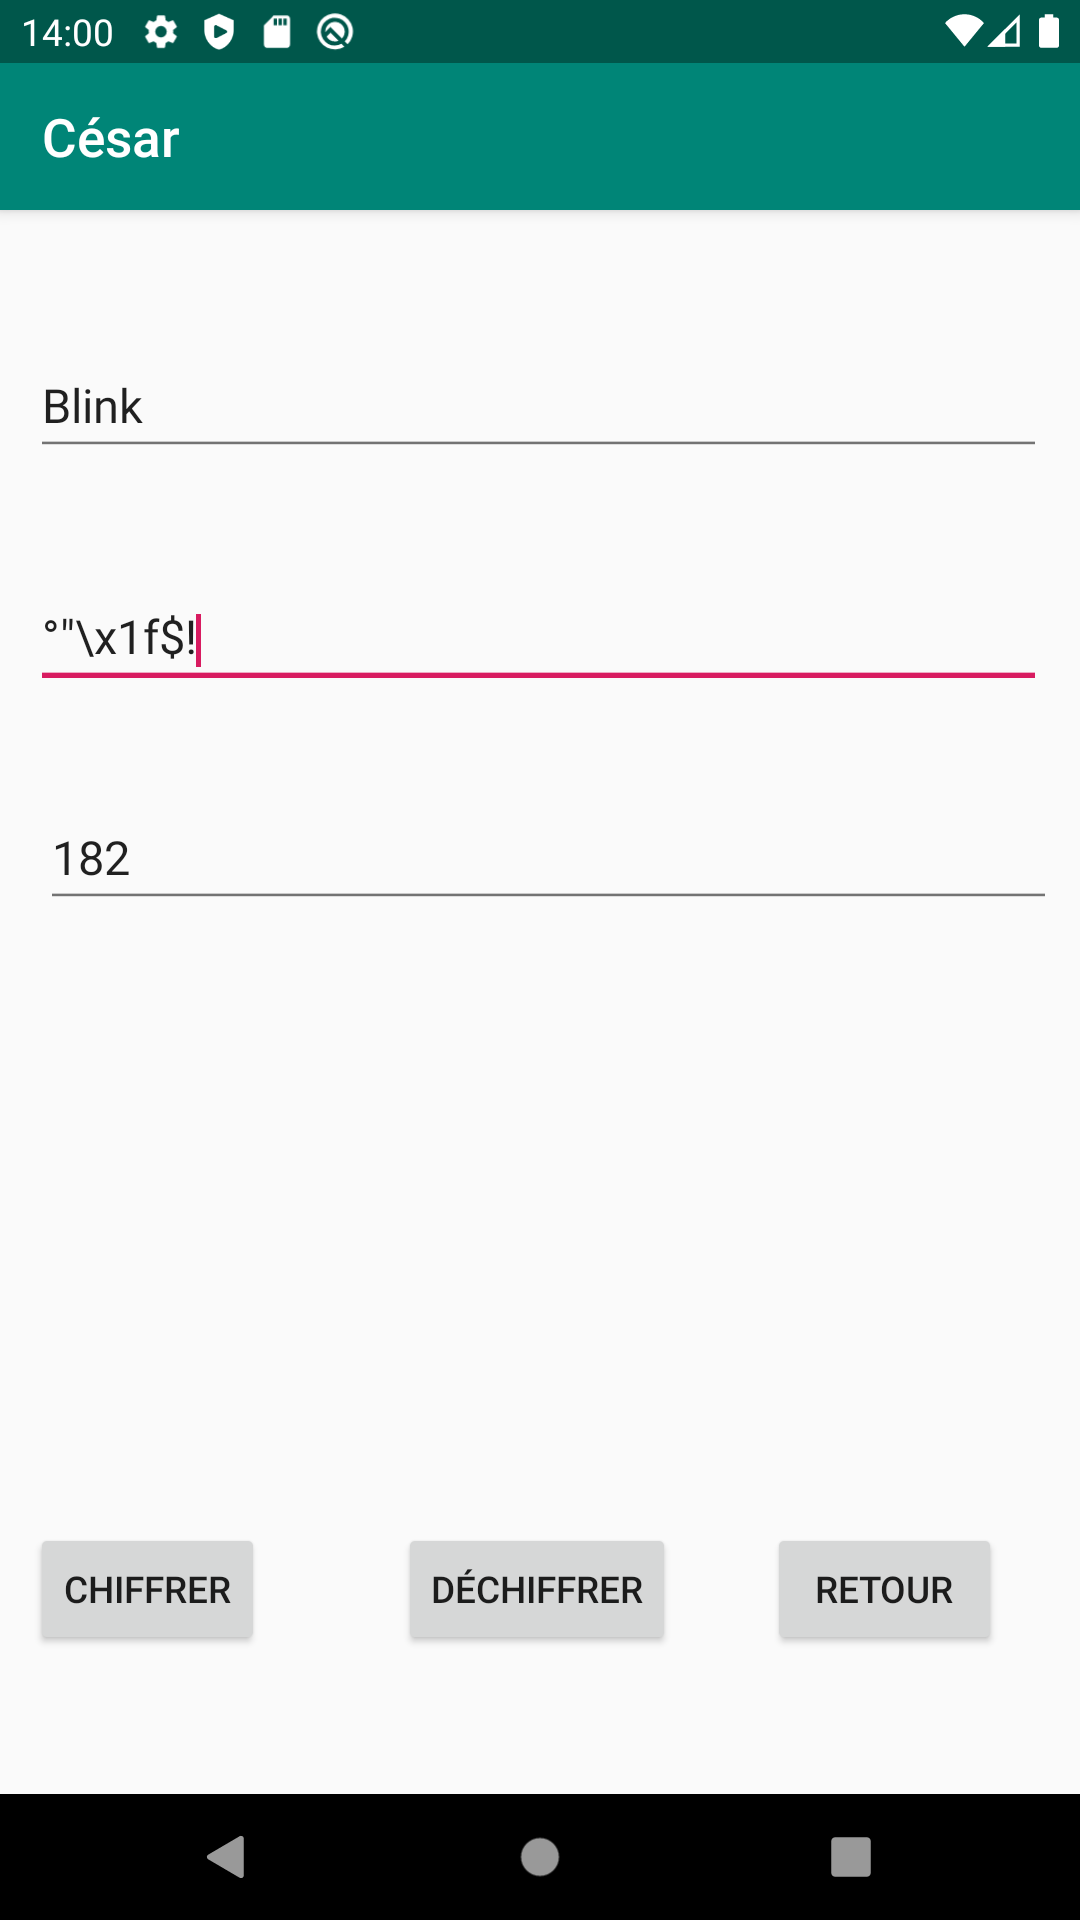
\includegraphics[width=.35\linewidth]{./img/cesar_e.png} &
      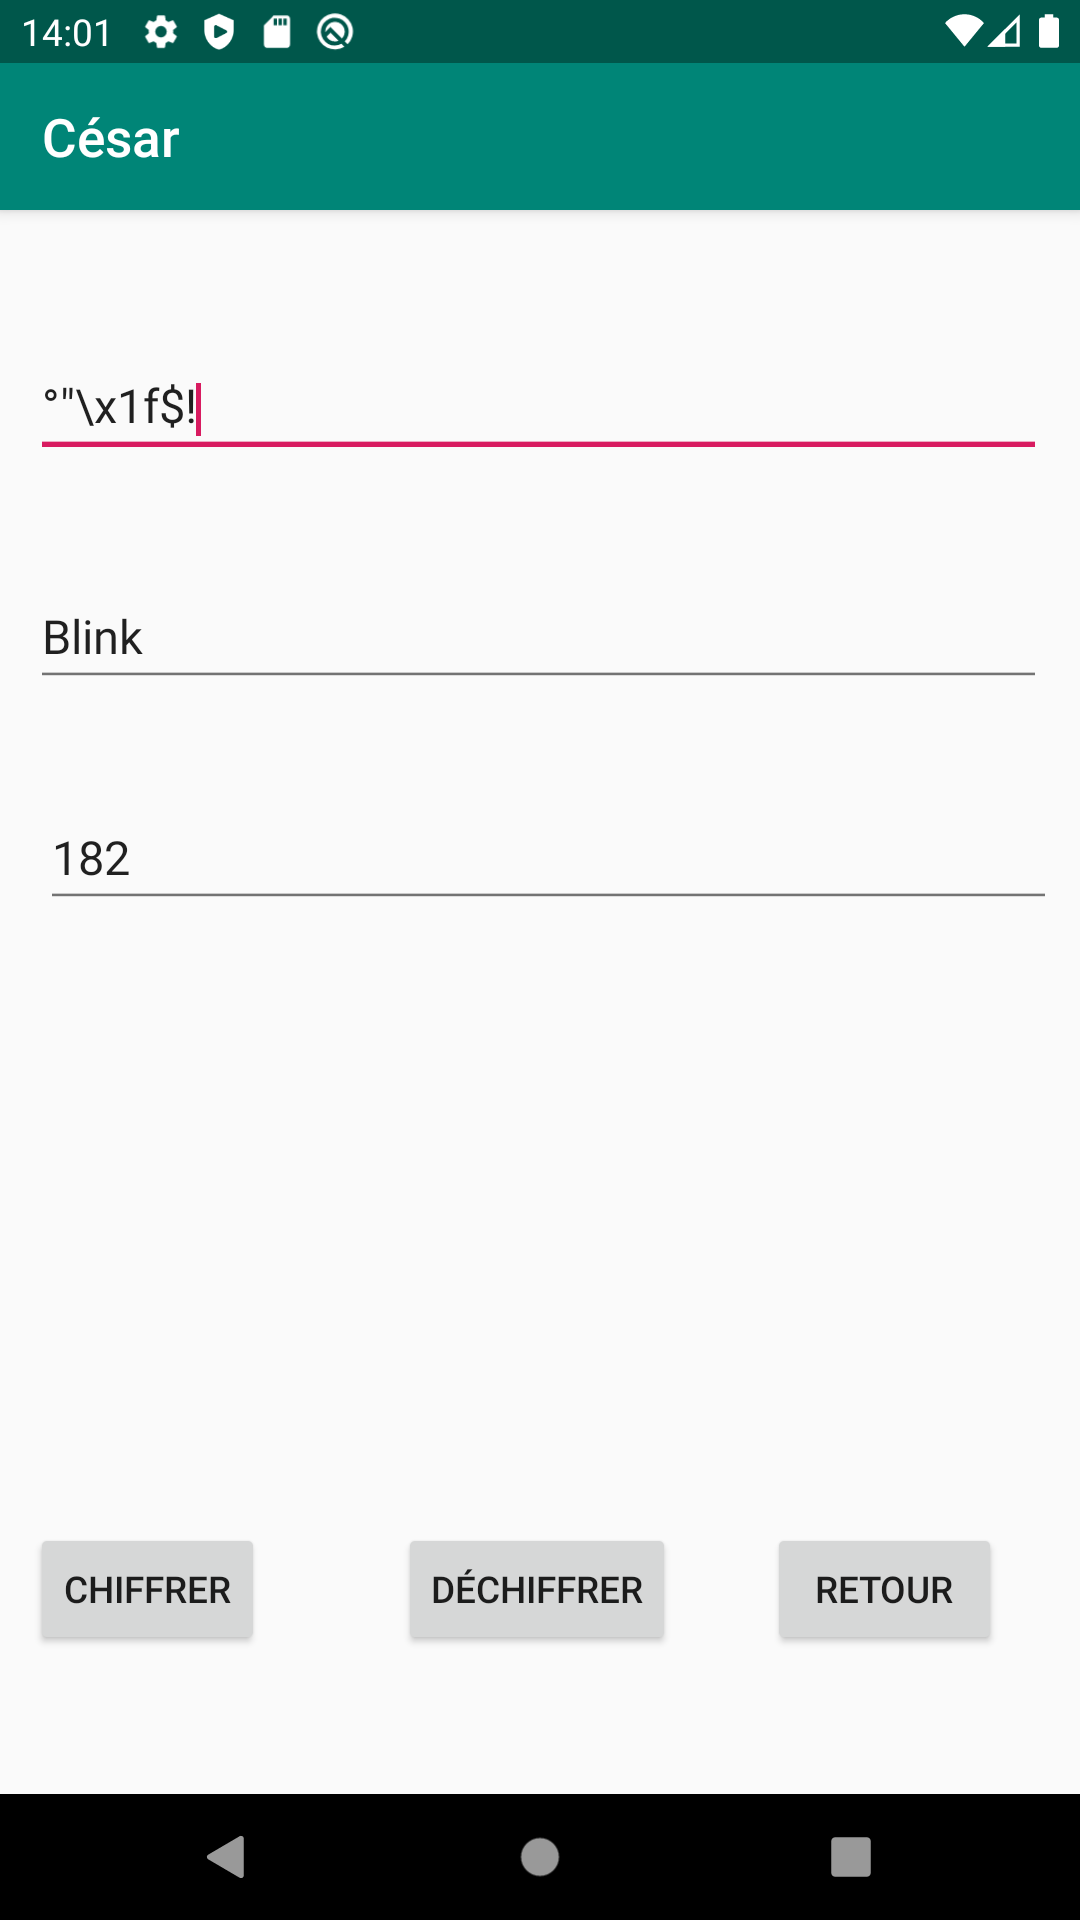
\includegraphics[width=.35\linewidth]{./img/cesar_d.png} \\
      Chiffrage de "Blink" avec d=182 & Déchiffrage de ""\textbackslash x1f \$ !" avec d=182\\
    \end{tabular}
    \caption{Chiffrage et déchiffrage avec \textbf{Cesar}}\label{fig:cesar}
\end{figure}

\begin{figure}[b!]
    \centering
    \begin{tabular}{cc}
      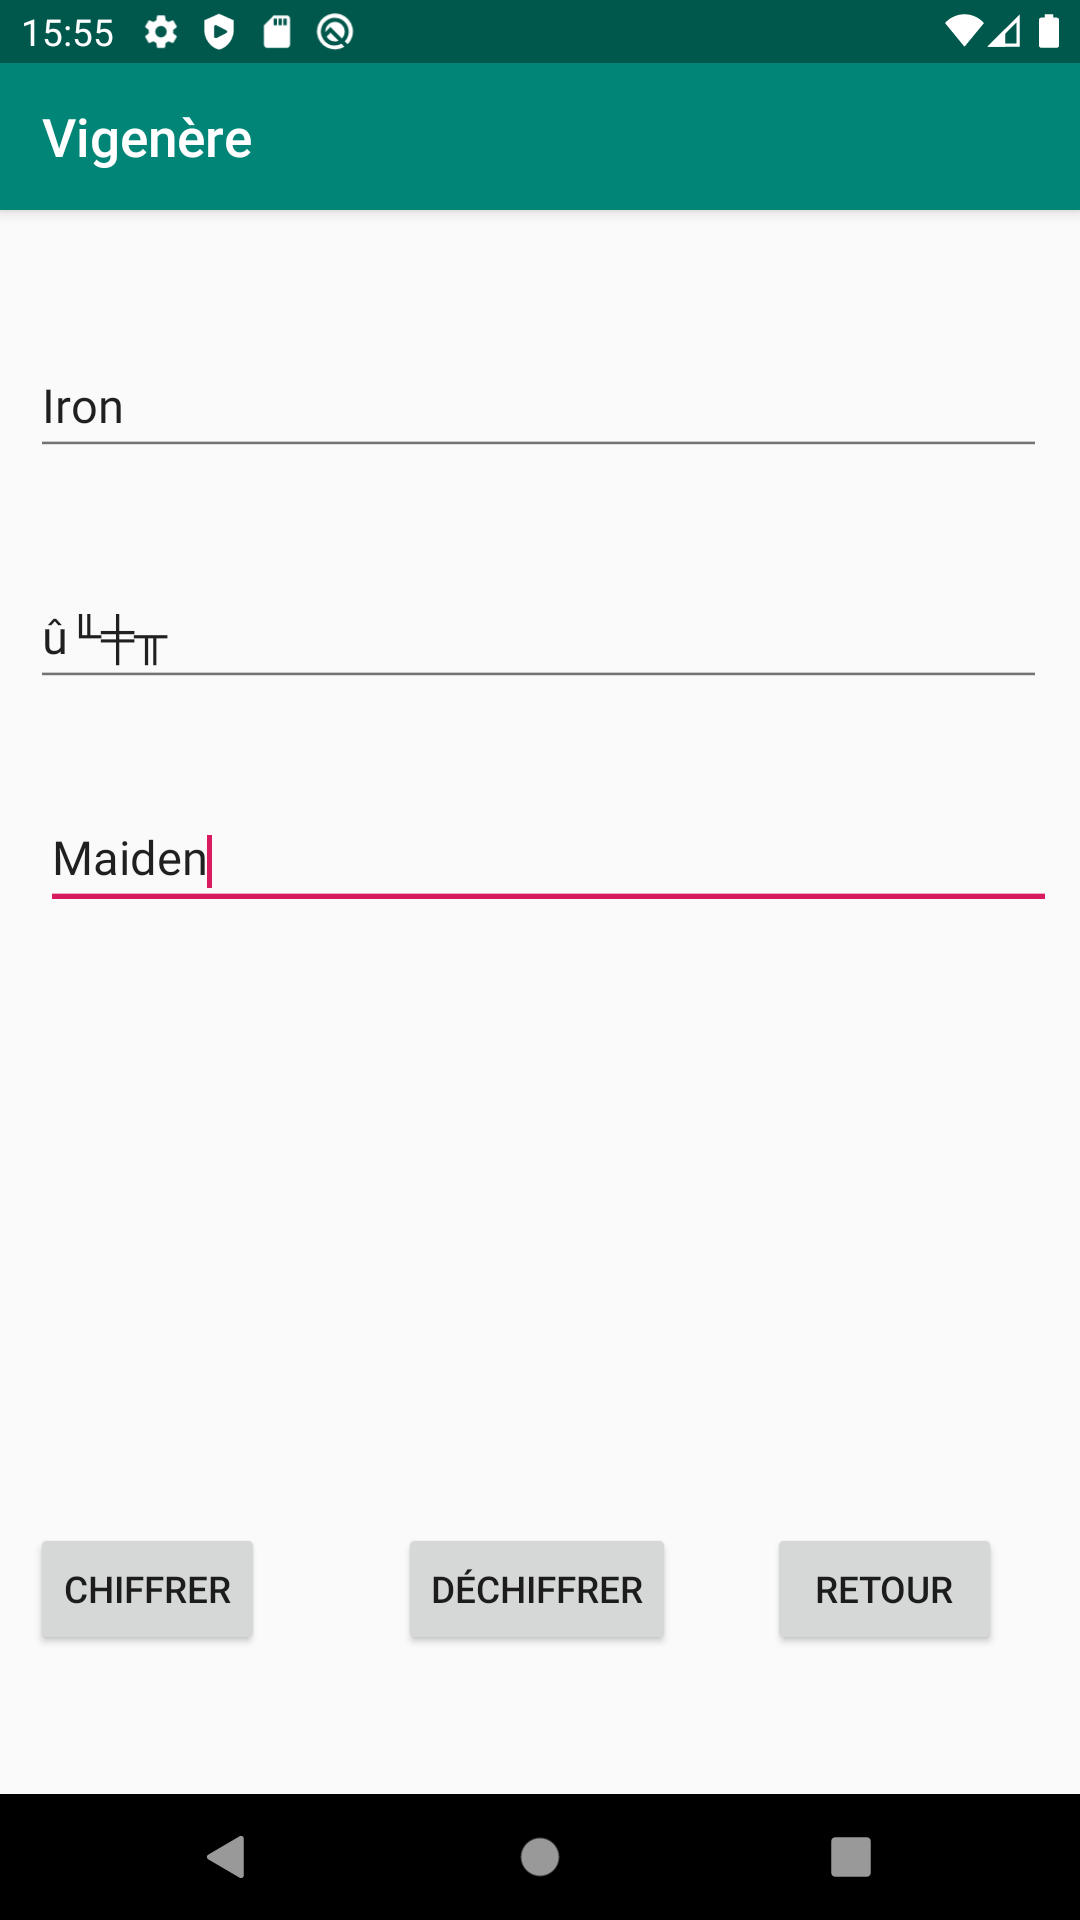
\includegraphics[width=.35\linewidth]{./img/vigenere_e.png} &
      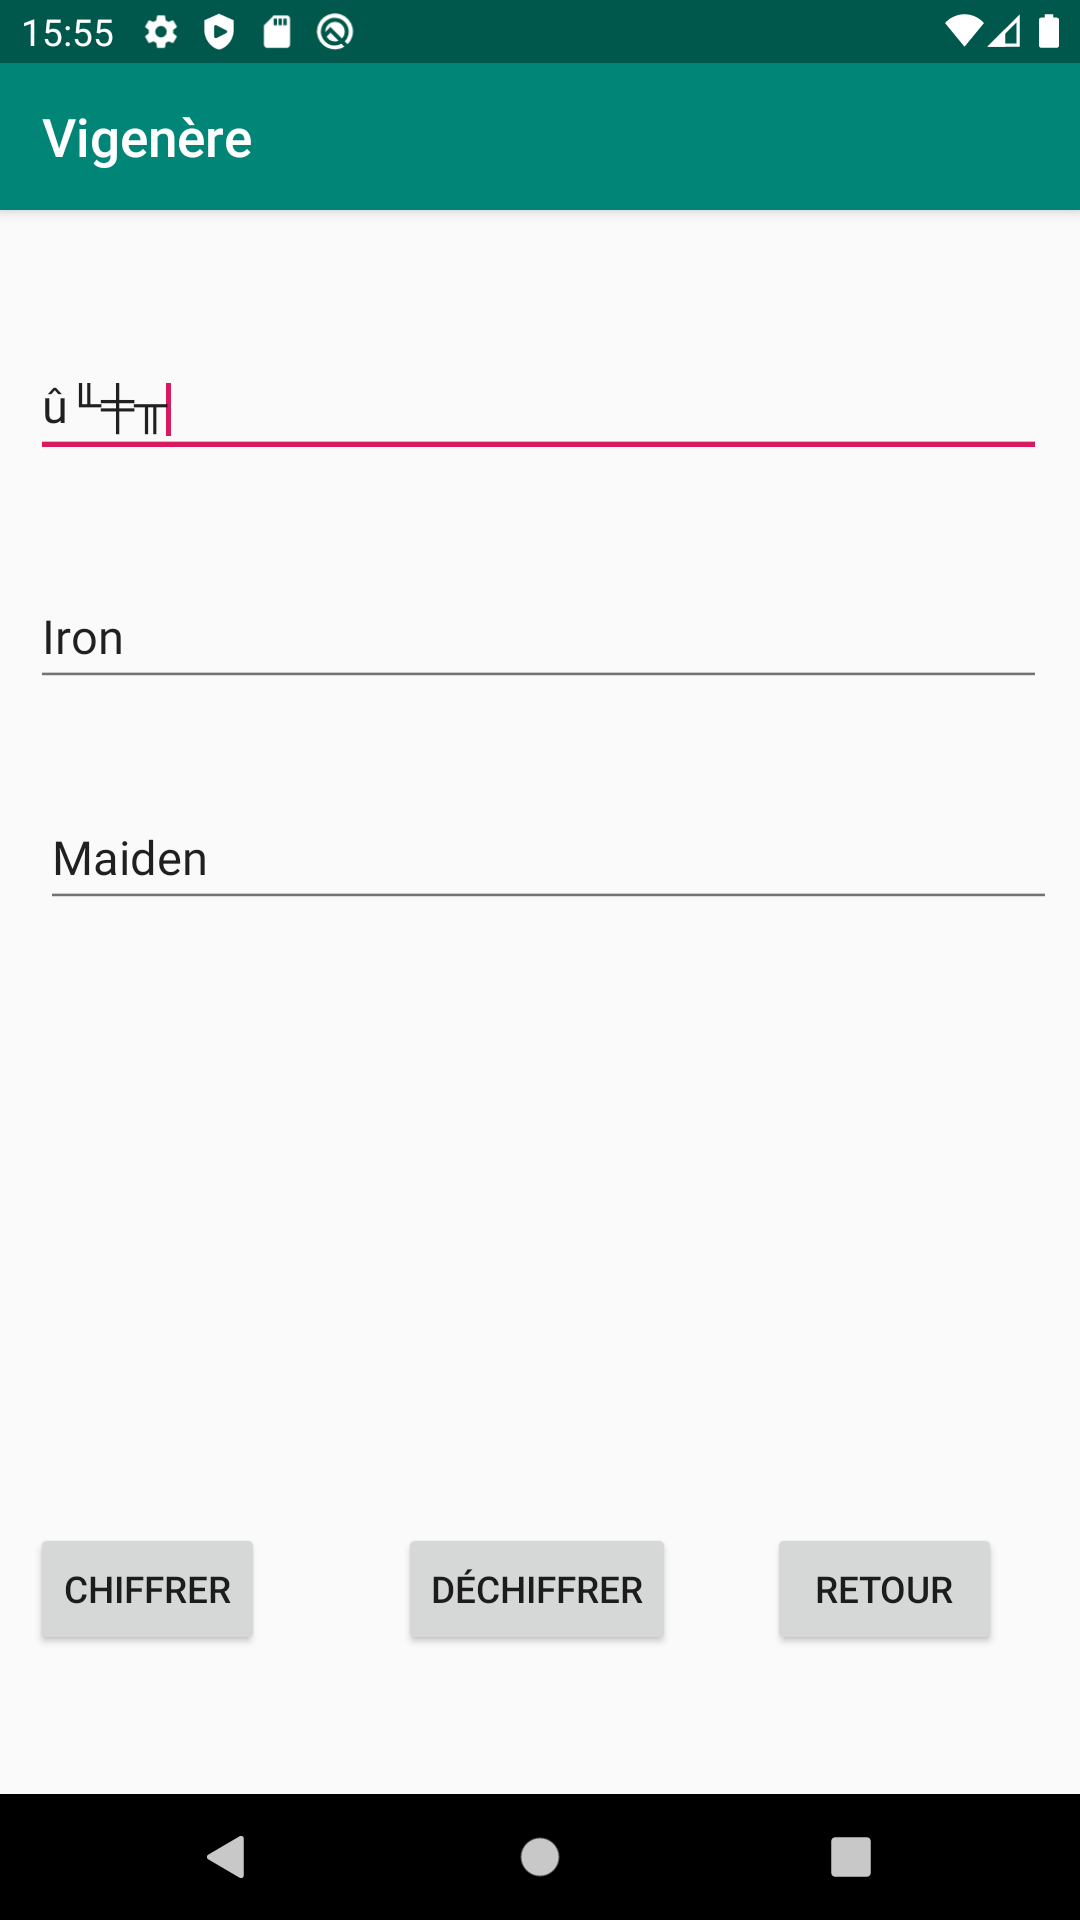
\includegraphics[width=.35\linewidth]{./img/vigenere_d.png} \\
      Chiffrage de "Iron" avec la clé "Maiden" & Déchiffrage \\
    \end{tabular}
    \caption{Chiffrage et déchiffrage avec \textbf{Vigenère}}\label{fig:vigenere}
\end{figure}

\begin{figure}[b!]
    \centering
    \begin{tabular}{cc}
      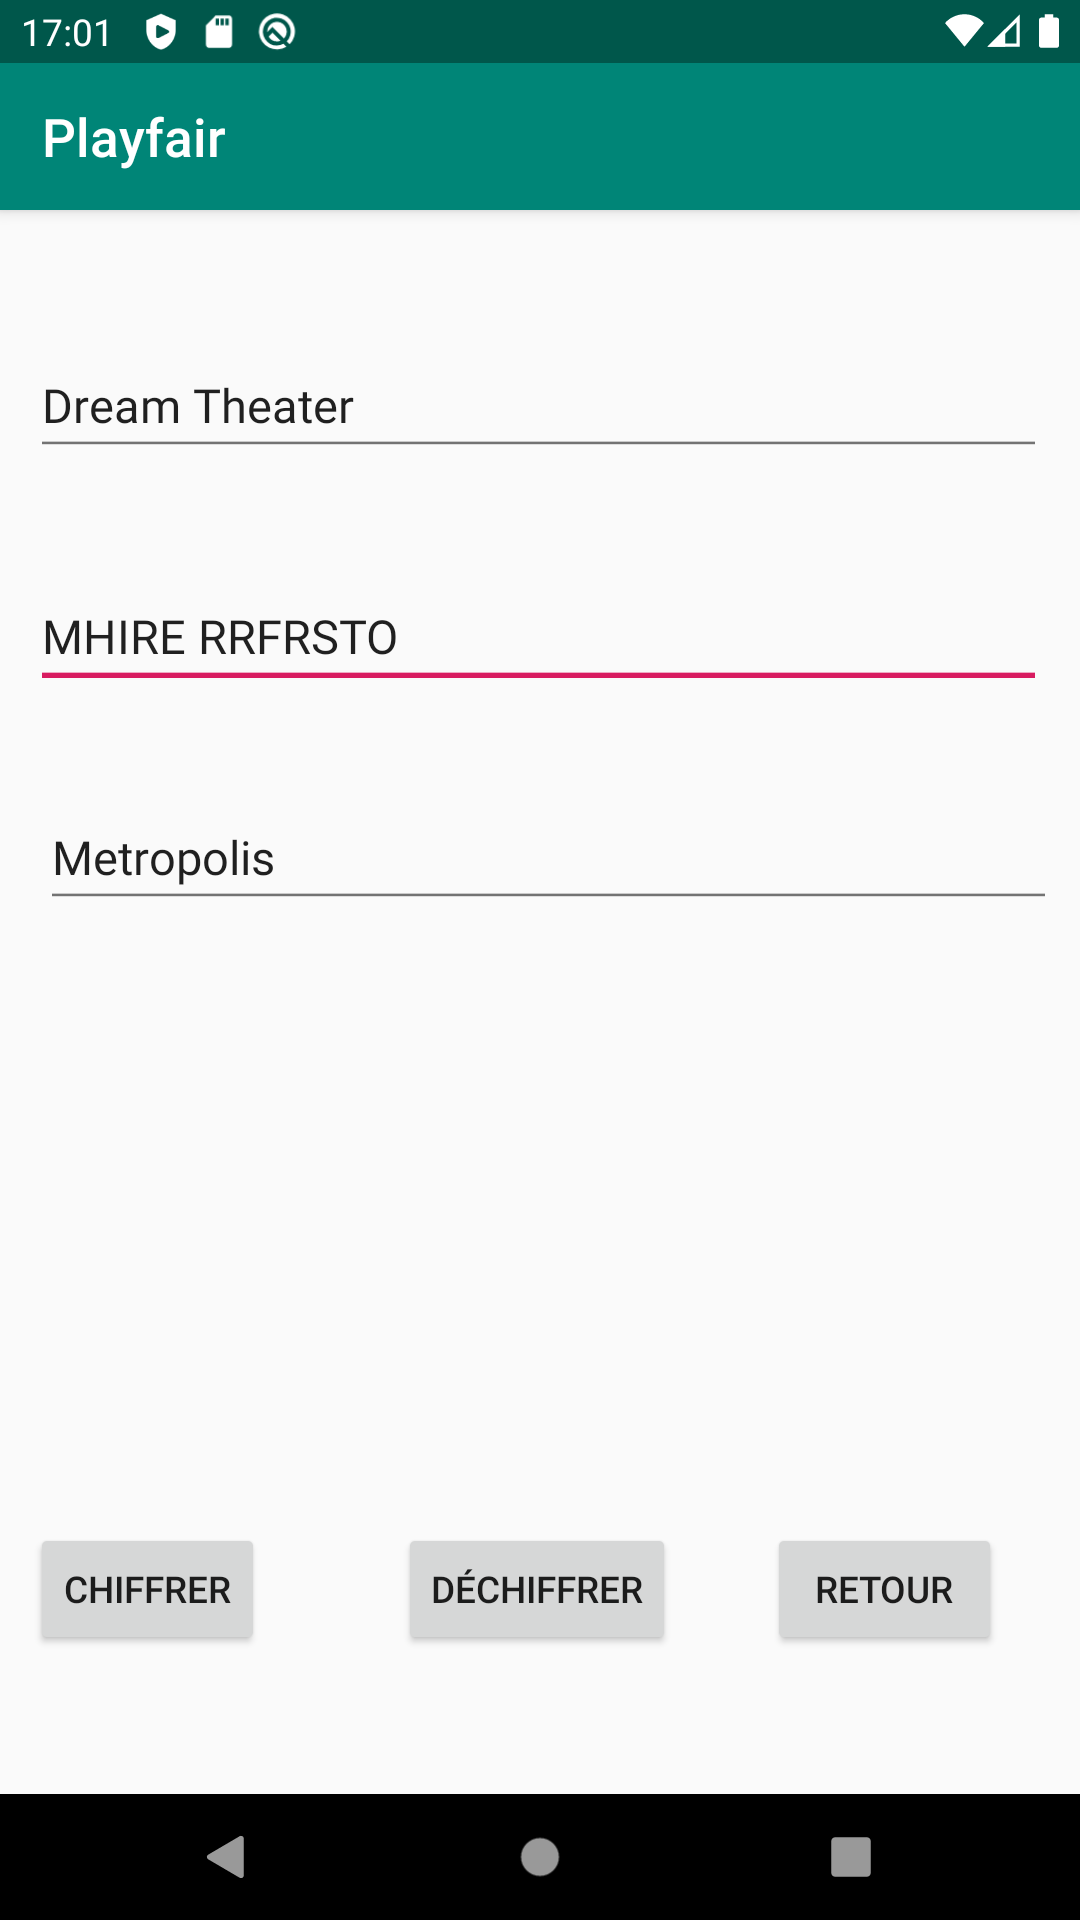
\includegraphics[width=.35\linewidth]{./img/playfair_e.png} &
      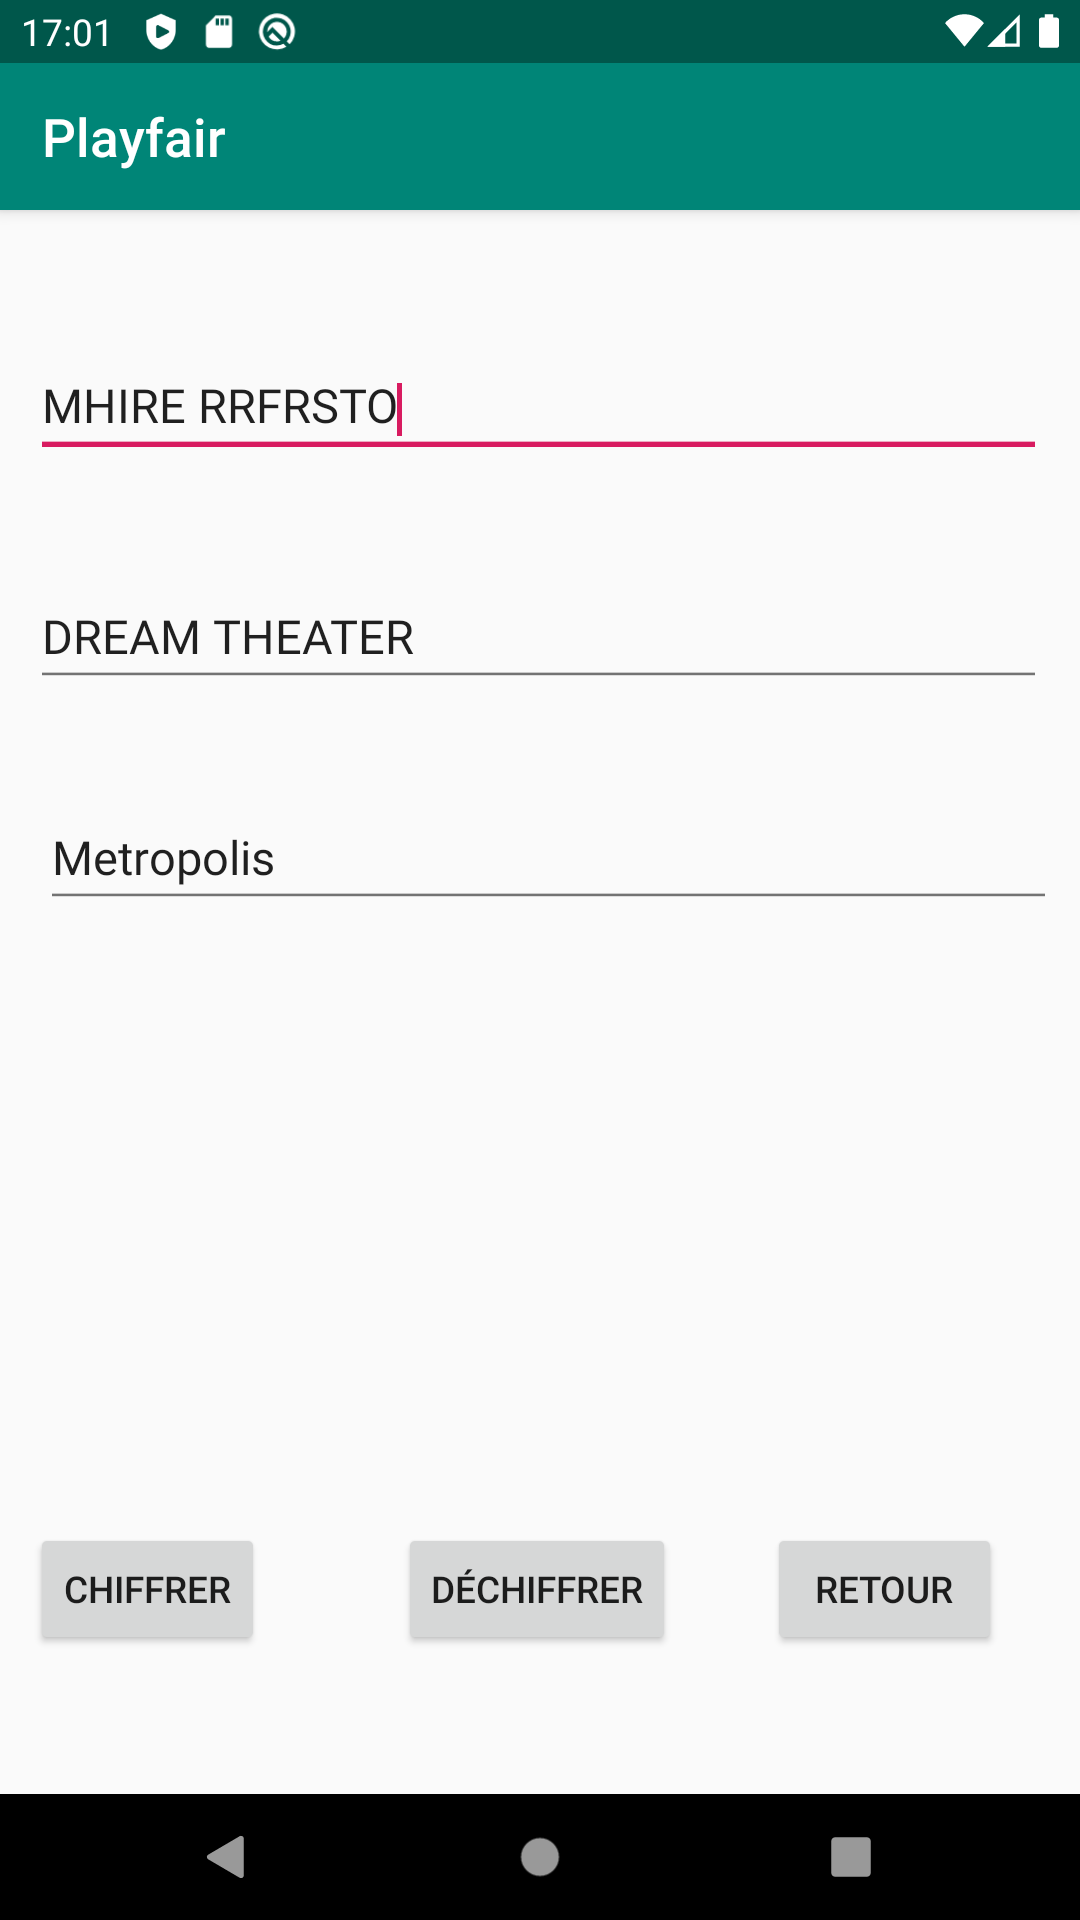
\includegraphics[width=.35\linewidth]{./img/playfair_d.png} \\
      Chiffrage de "Dream Theater" avec la clé "Metropolis" & Déchiffrage de "MHIRE RRFRSTO"\\
    \end{tabular}
    \caption{Chiffrage et déchiffrage avec \textbf{Playfair}}\label{fig:playfair}
\end{figure}

\begin{figure}[b!]
    \centering
    \begin{tabular}{cc}
      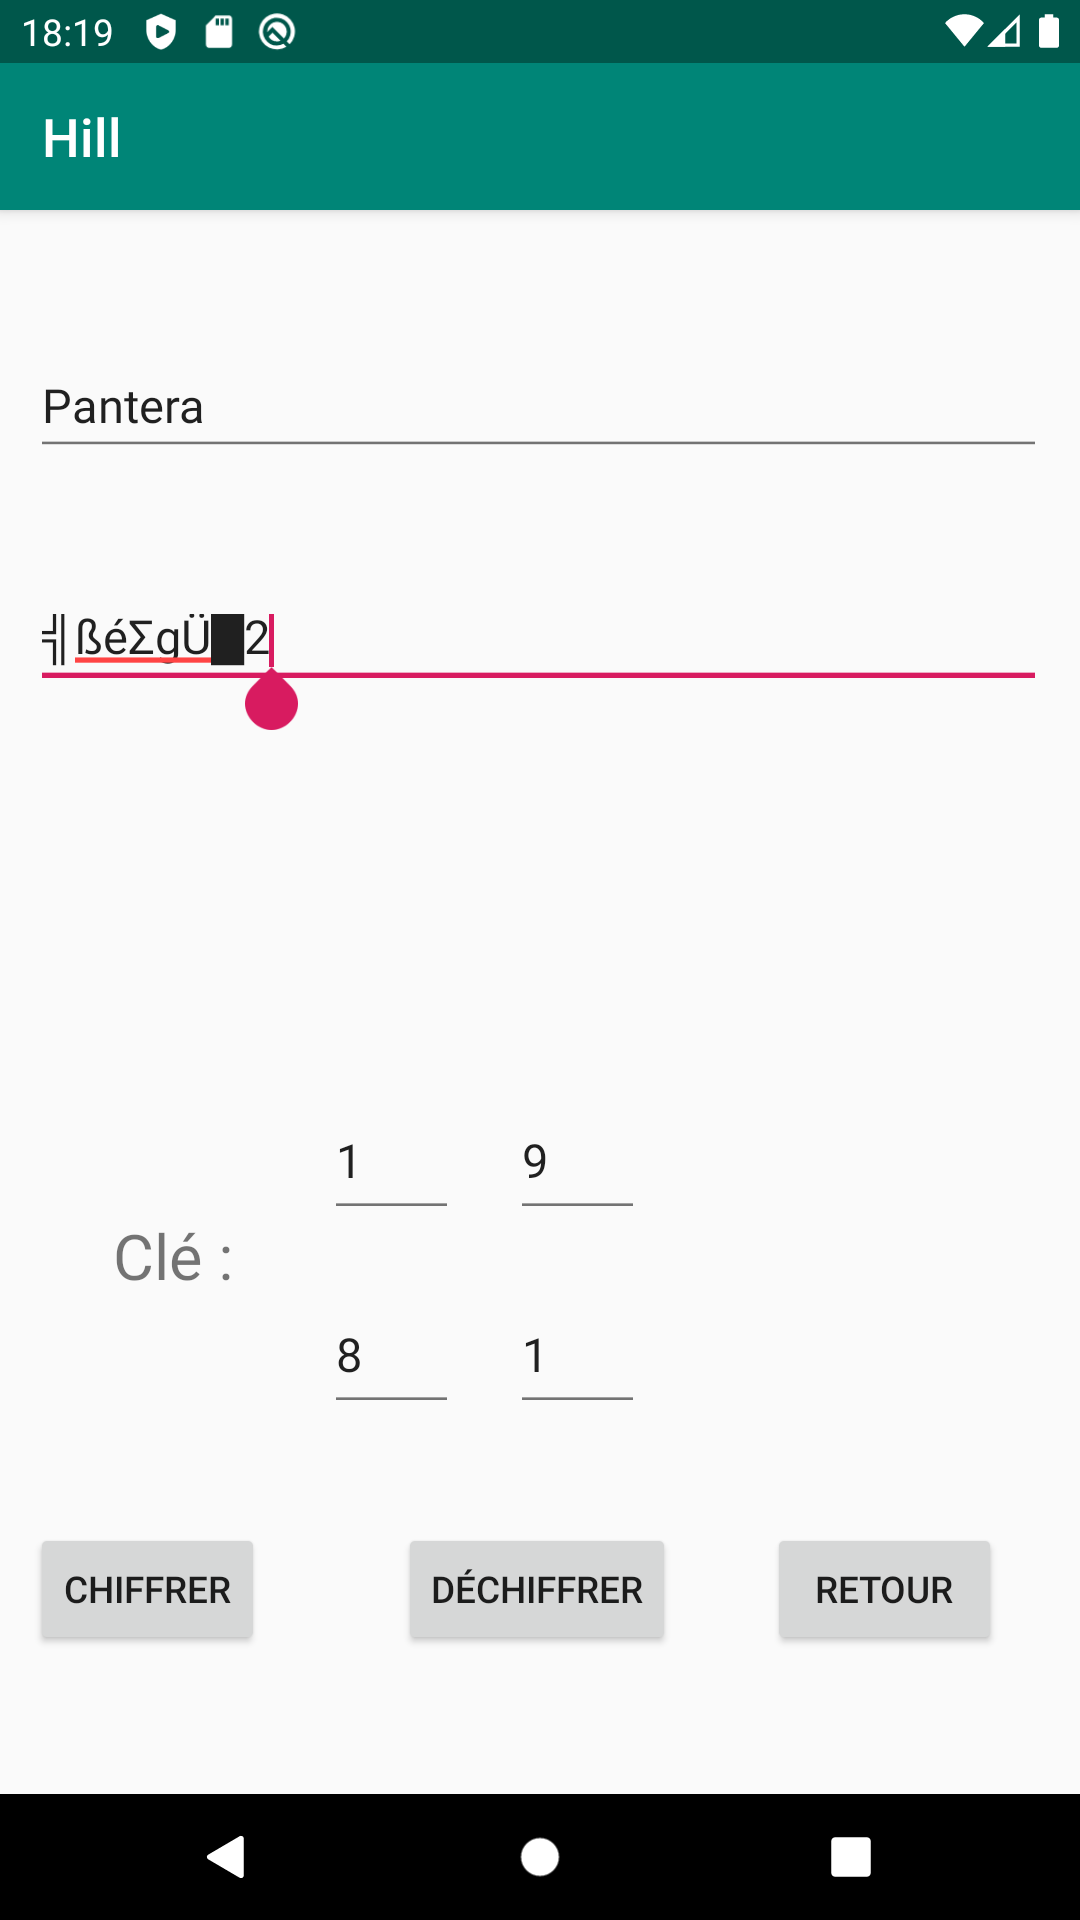
\includegraphics[width=.35\linewidth]{./img/hill_e.png} &
      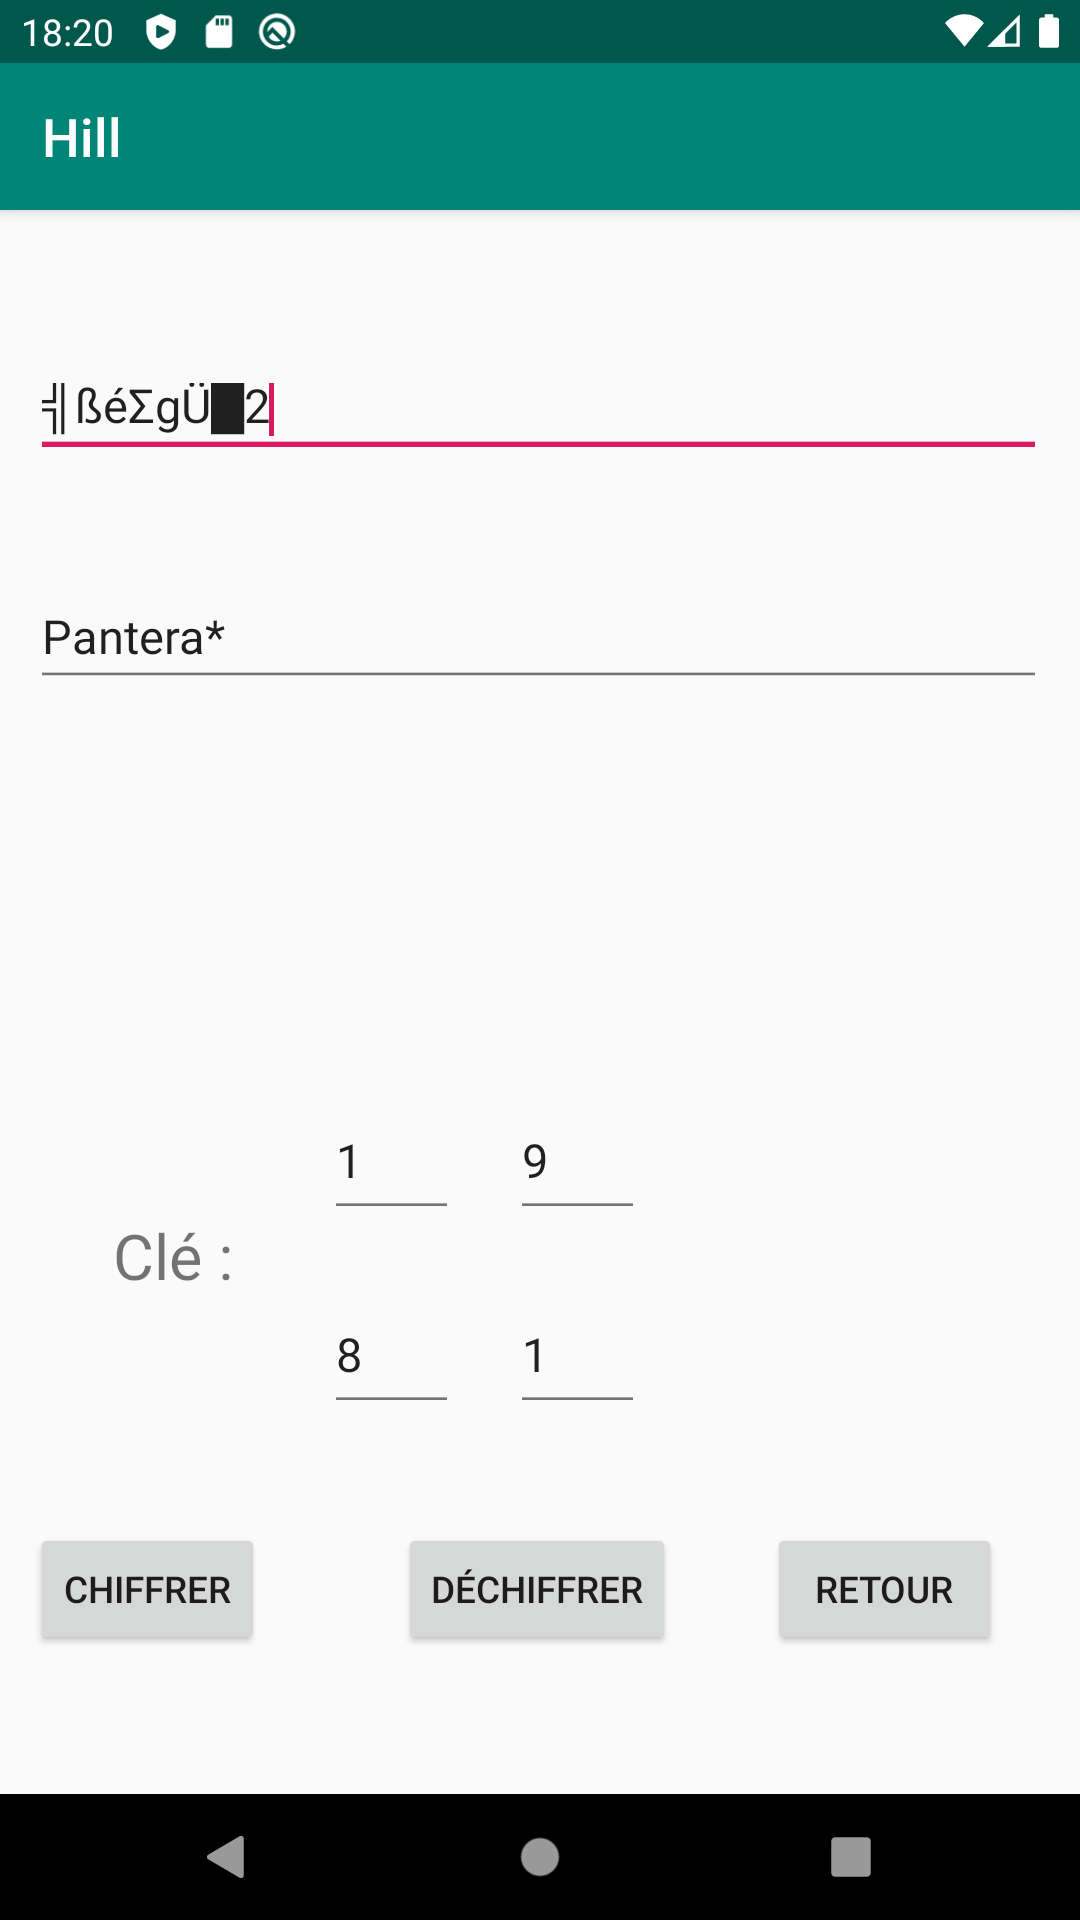
\includegraphics[width=.35\linewidth]{./img/hill_d.png} \\
      Chiffrage de "Pantera" avec la clé $\begin{pmatrix}
1&9\\
8&1\\
\end{pmatrix}$ & Déchiffrage\\
    \end{tabular}
    \caption{Chiffrage et déchiffrage avec \textbf{Hill}}\label{fig:hill}
\end{figure}

\begin{figure}[b!]
    \centering
    \begin{tabular}{cc}
      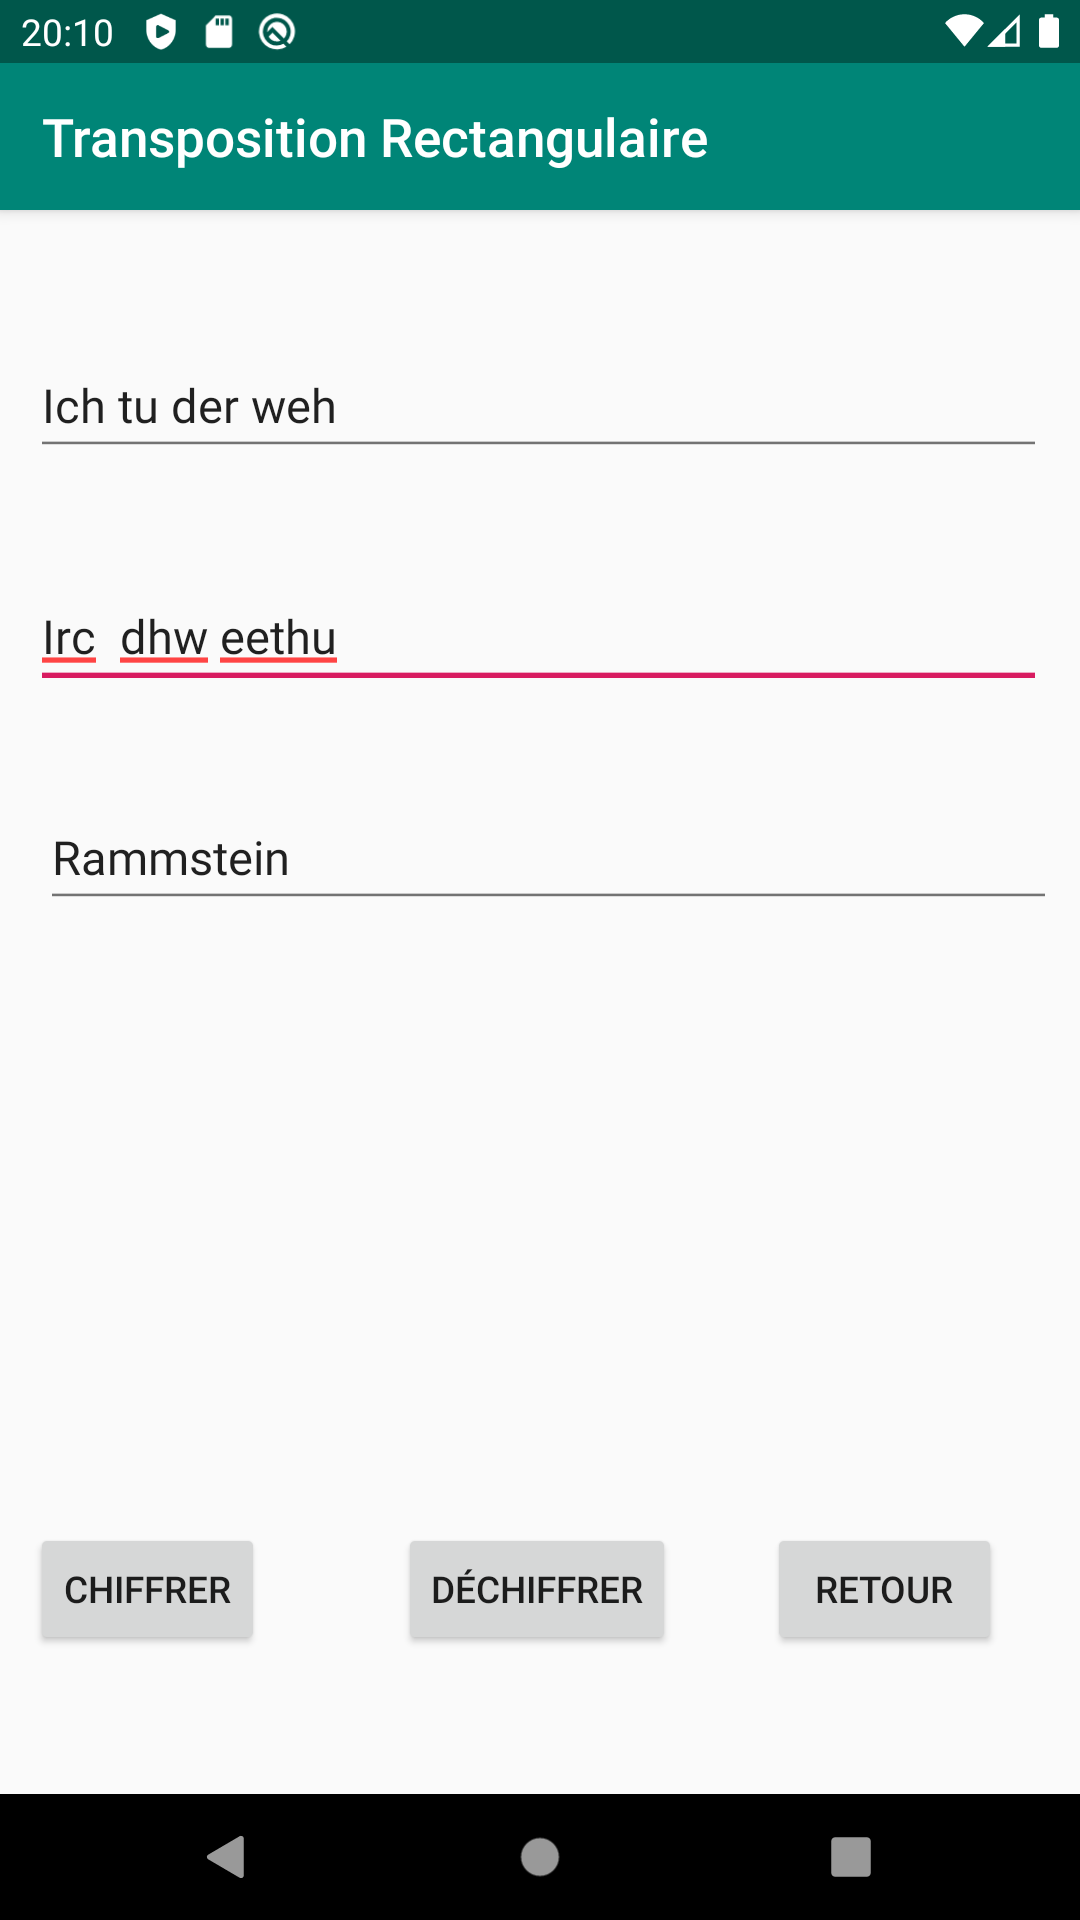
\includegraphics[width=.35\linewidth]{./img/transpo_e.png} &
      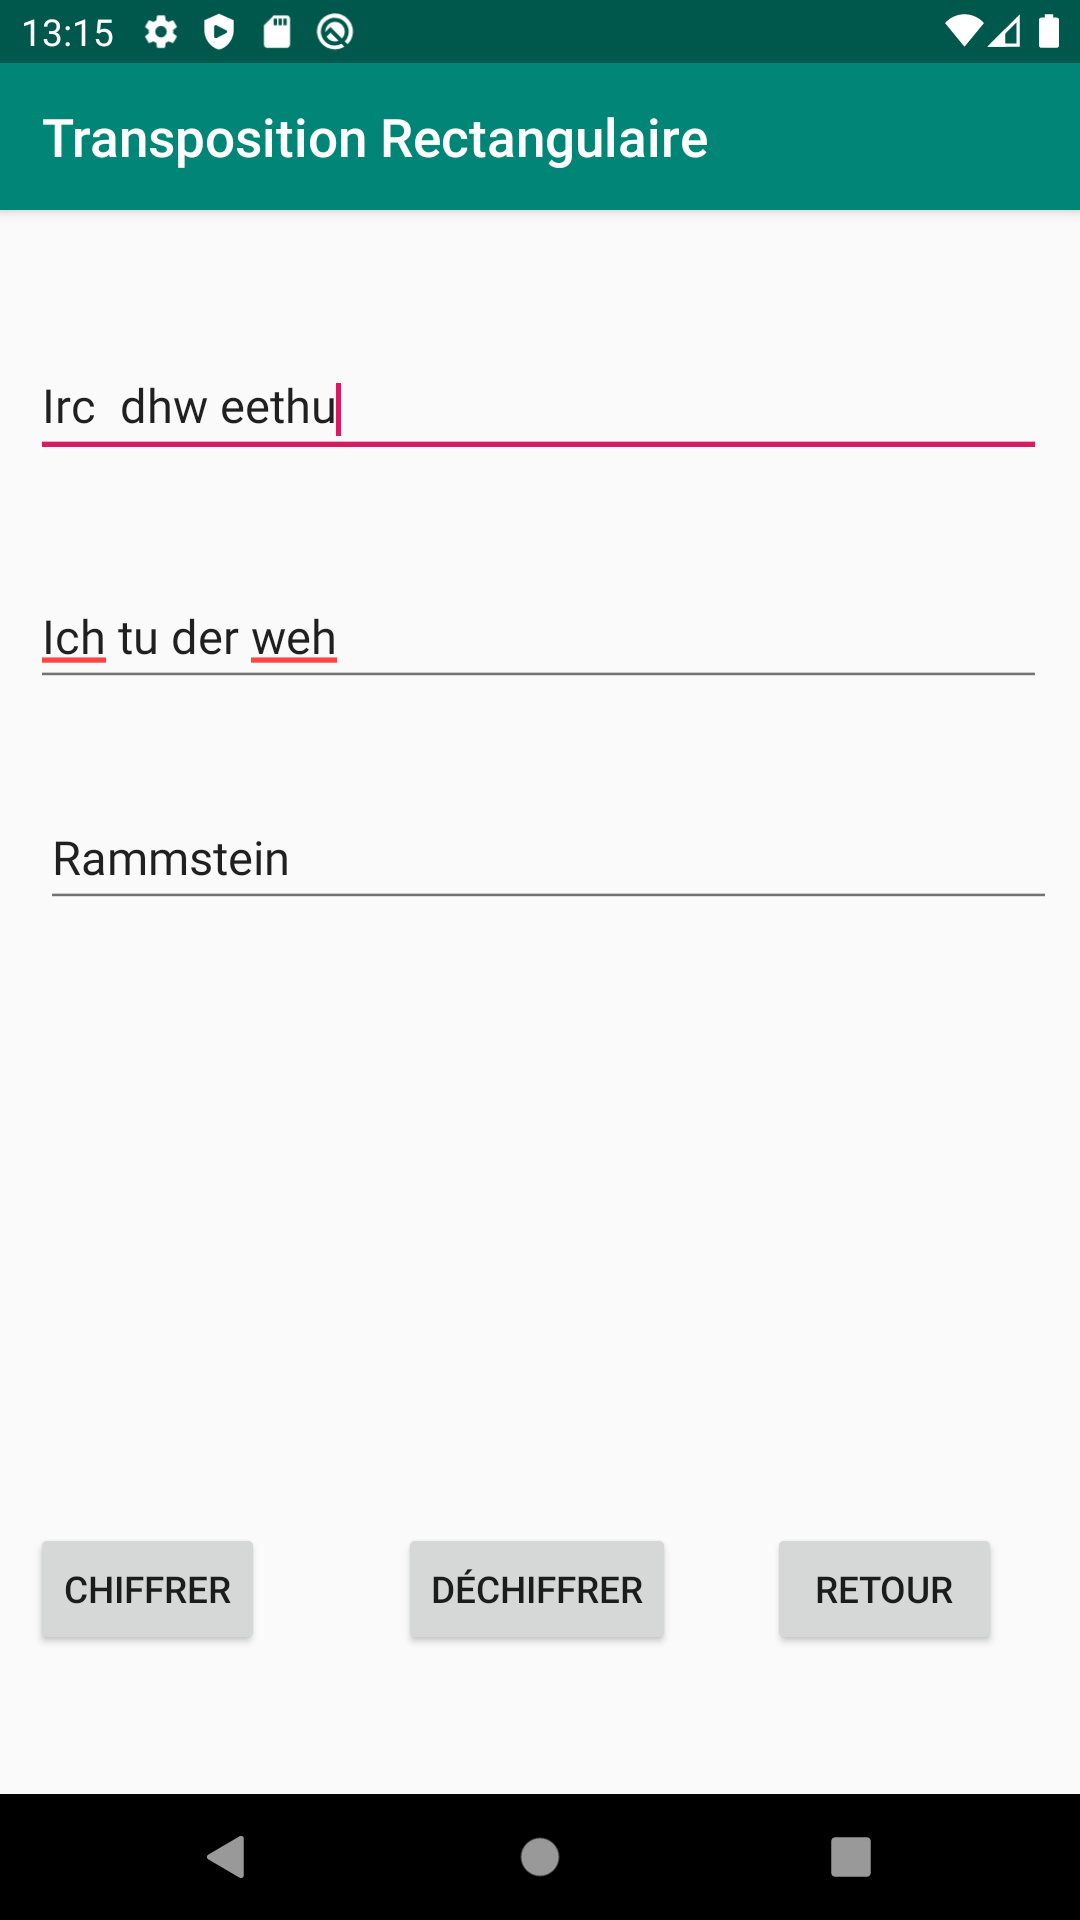
\includegraphics[width=.35\linewidth]{./img/transpo_d.png} \\
      Chiffrage de "Ich tu der weh" avec la clé "Rammstein" & Déchiffrage \\
    \end{tabular}
    \caption{Chiffrage et déchiffrage avec une \textbf{Transposition Rectangulaire}}\label{fig:transpo}
\end{figure}

\begin{figure}[b!]
    \centering
    \begin{tabular}{cc}
      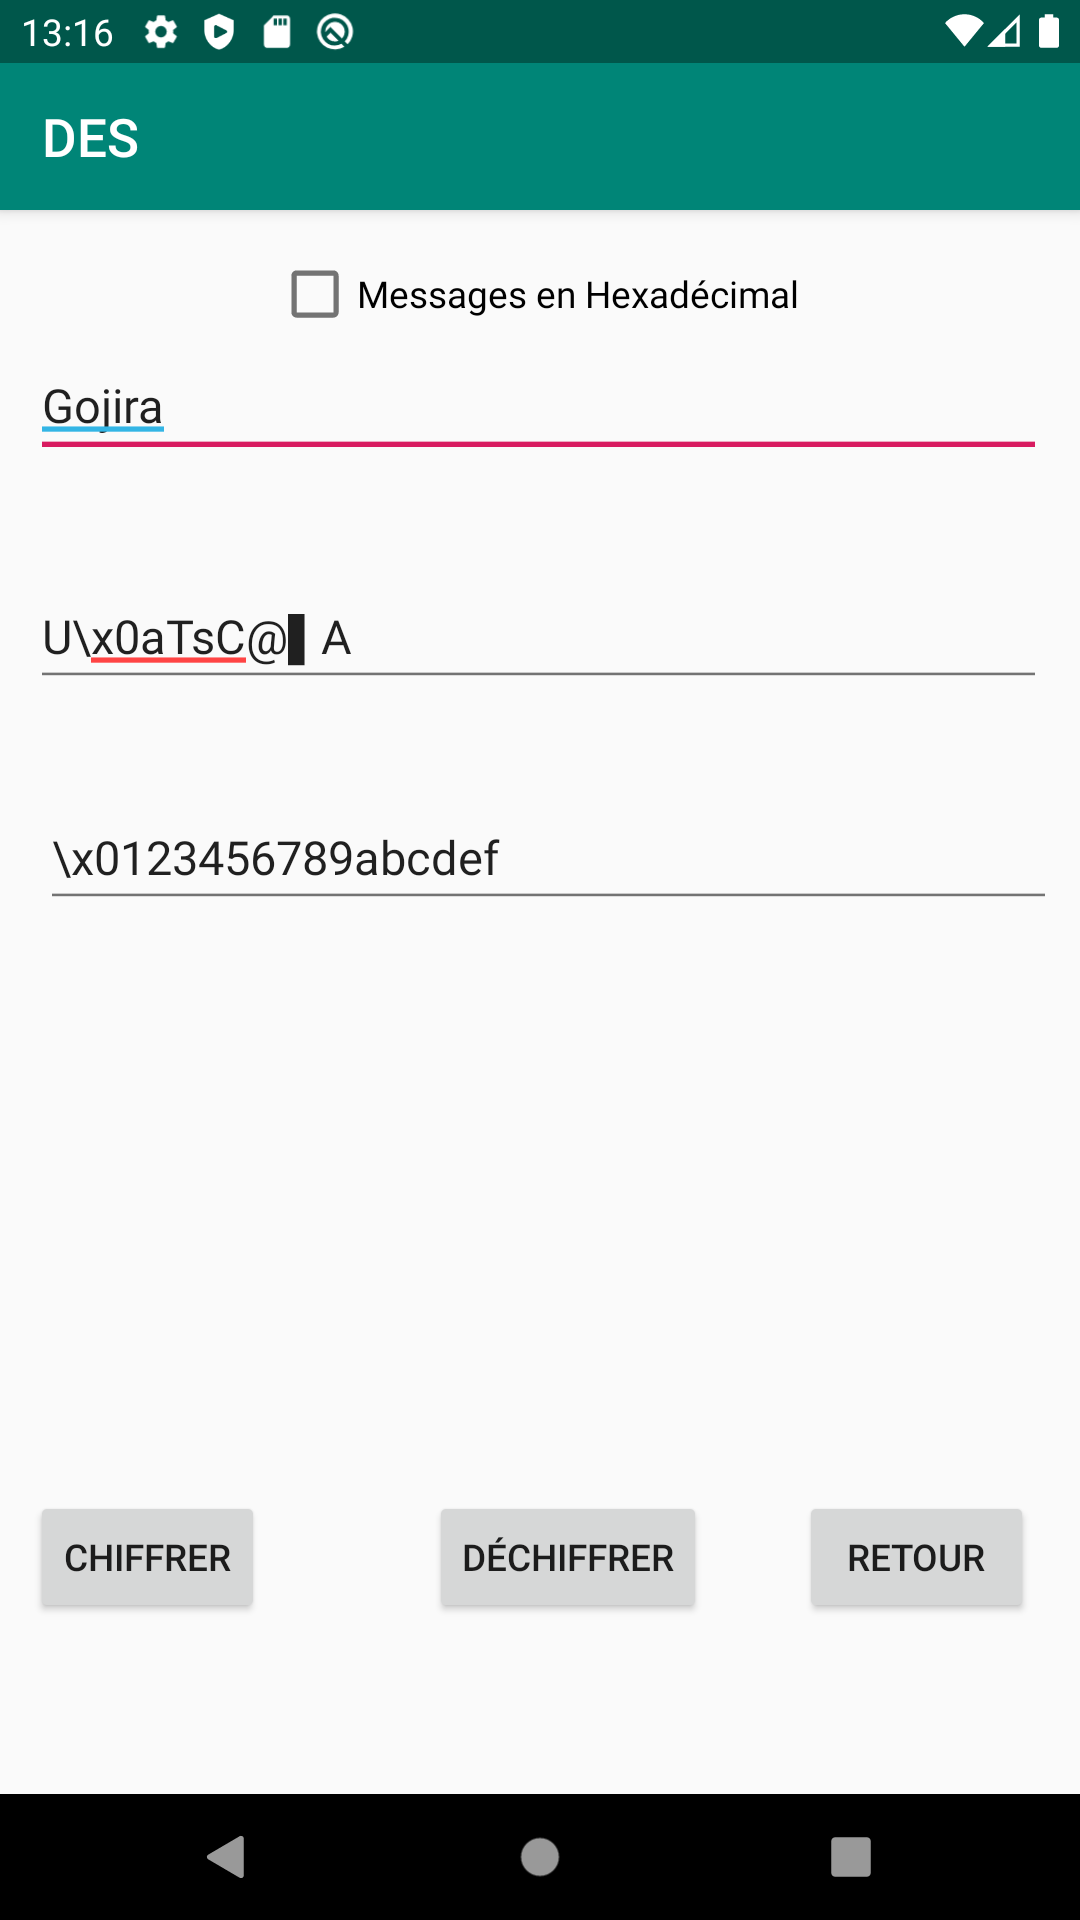
\includegraphics[width=.35\linewidth]{./img/des_e.png} &
      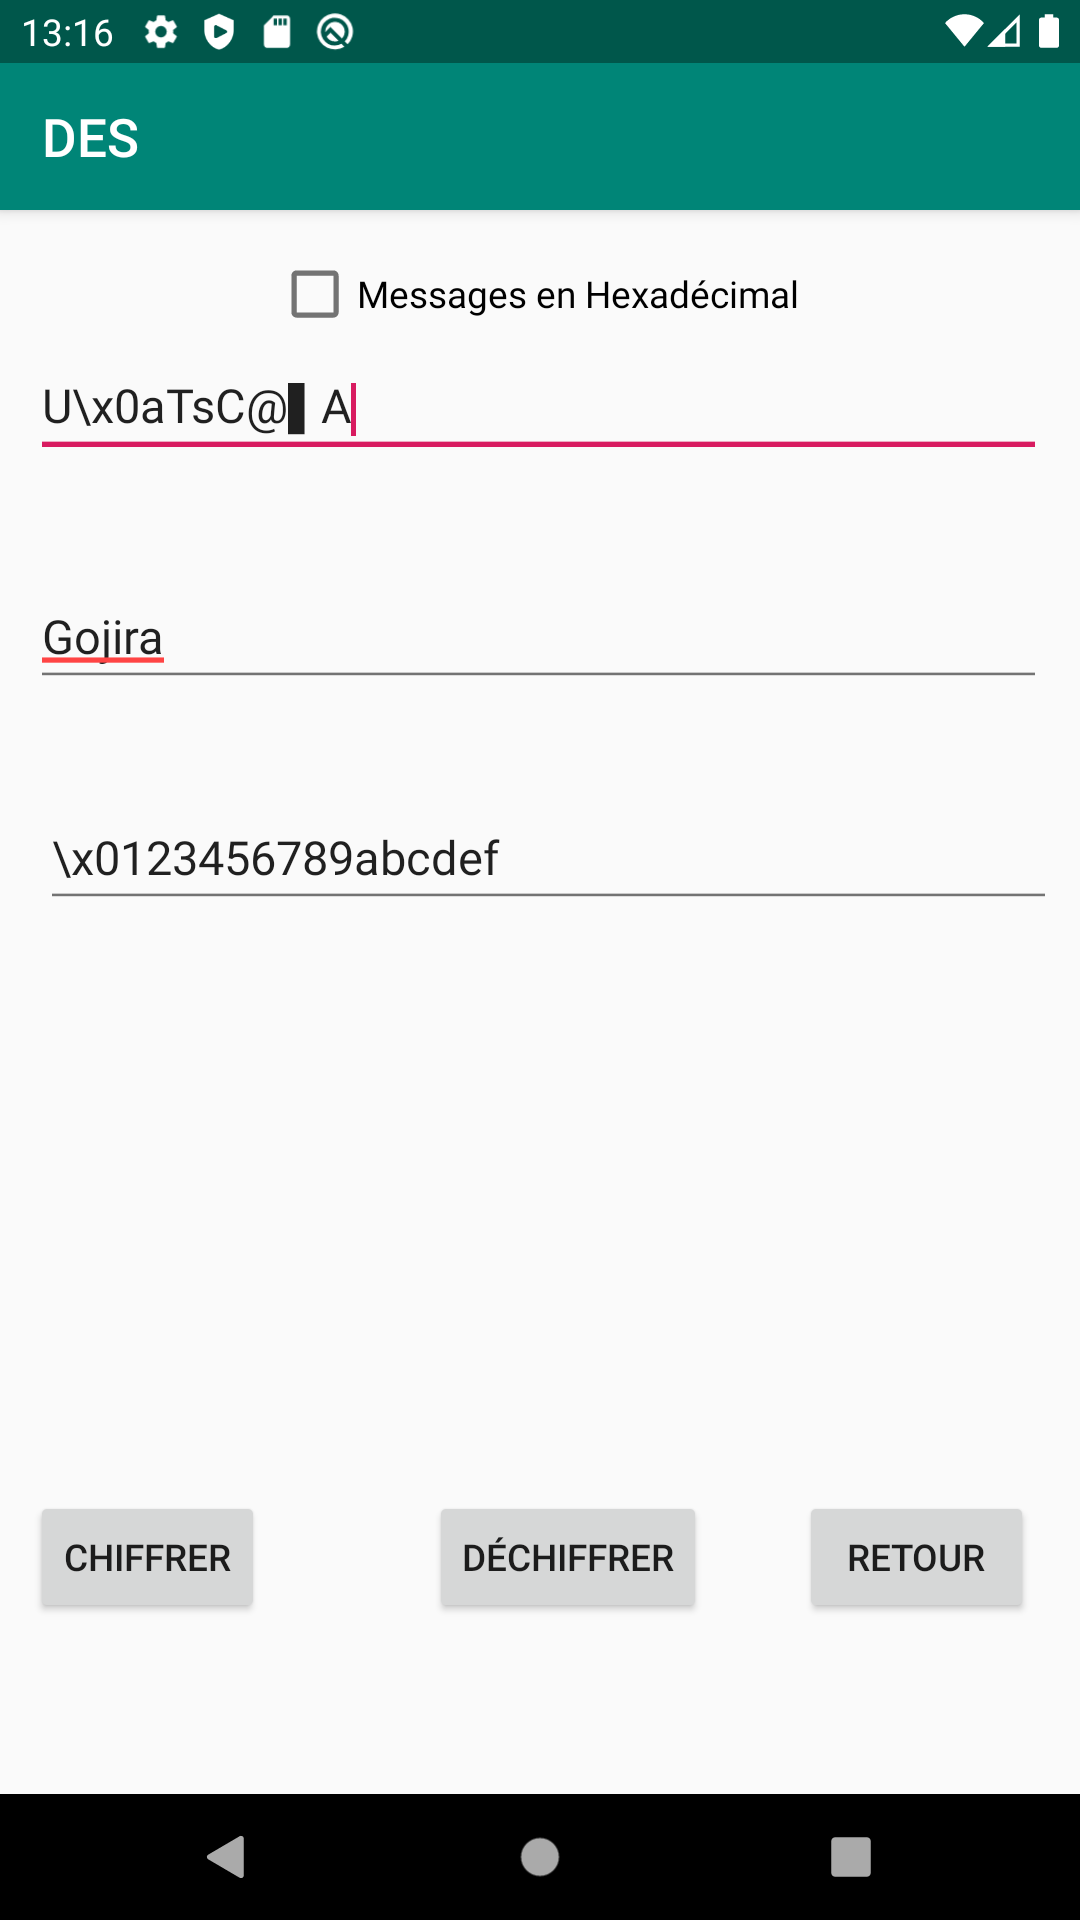
\includegraphics[width=.35\linewidth]{./img/des_d.png} \\
      Chiffrage de "Gojira" avec la clé "\textbackslash x0123456789abcdef" & Déchiffrage \\
    \end{tabular}
    \caption{Chiffrage et déchiffrage avec le \textbf{DES}}\label{fig:des}
\end{figure}

\begin{figure}[b!]
    \centering
    \begin{tabular}{cc}
      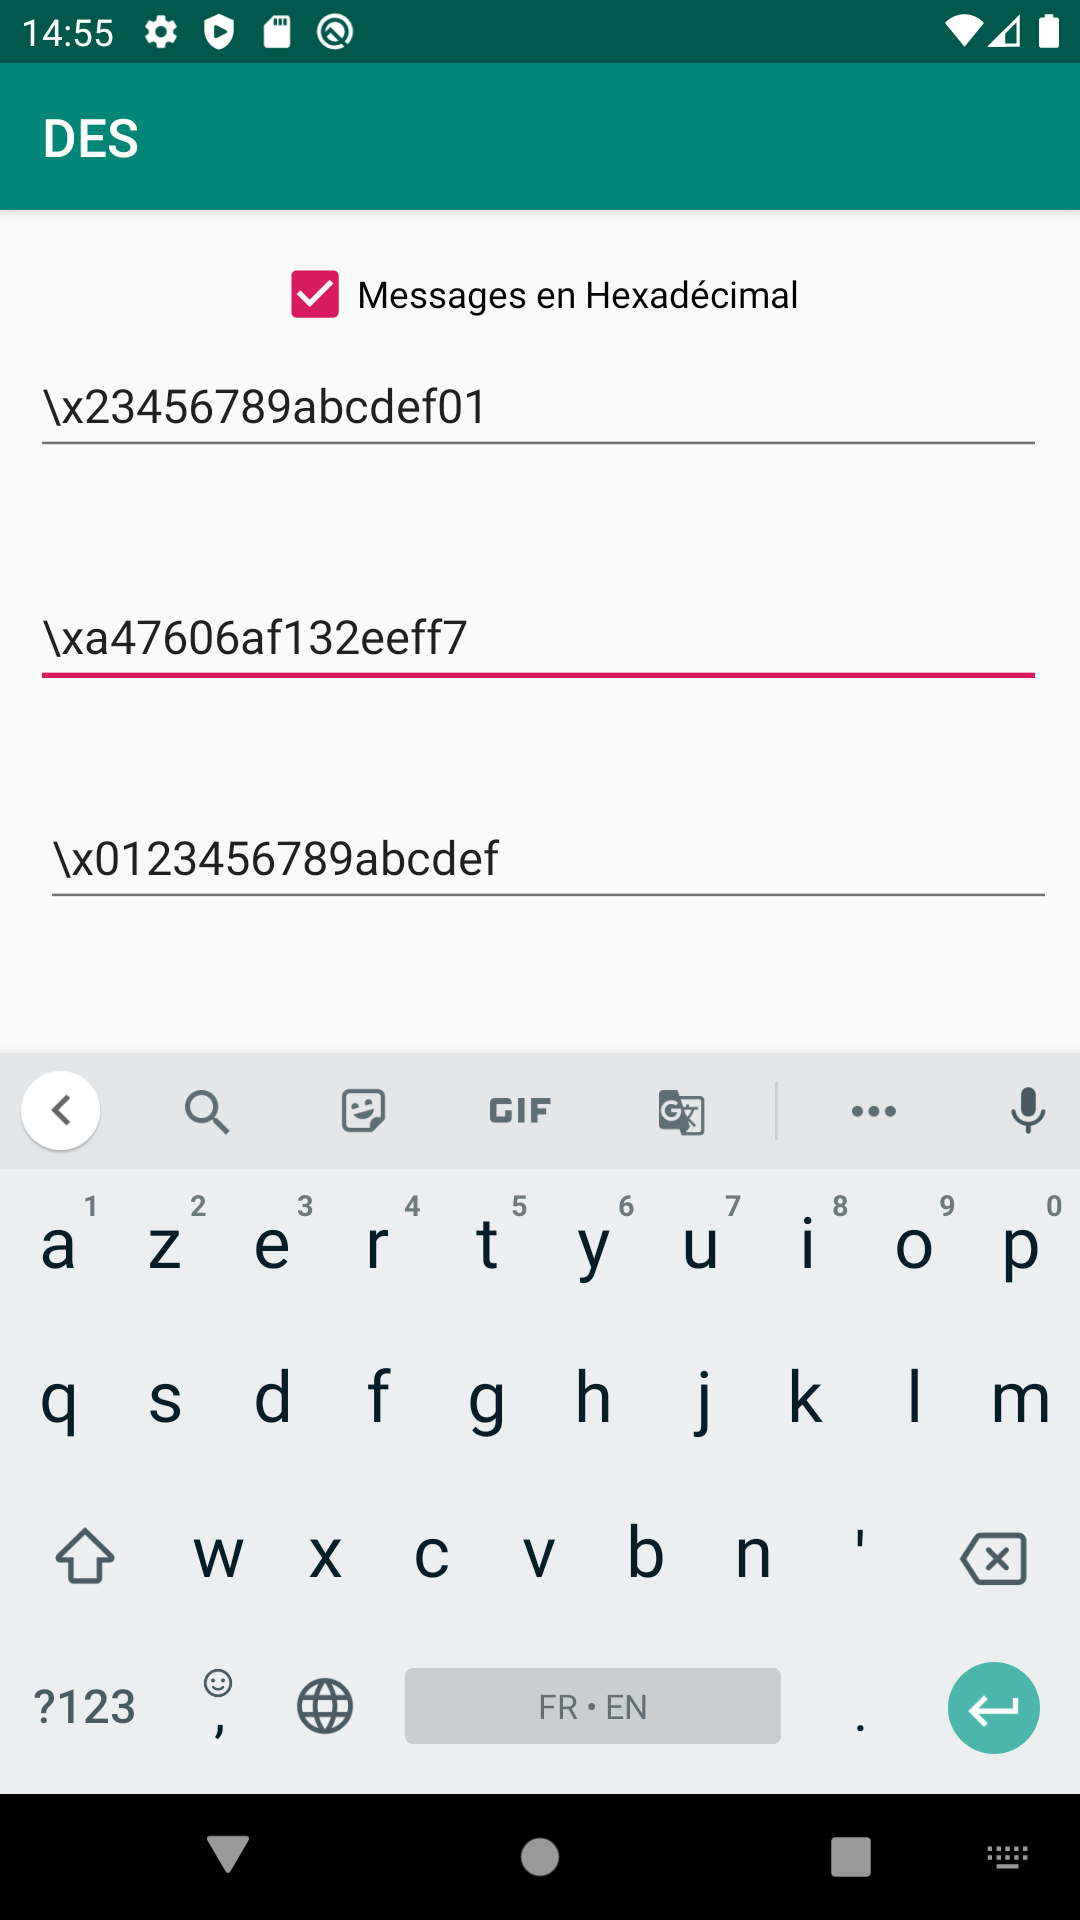
\includegraphics[width=.35\linewidth]{./img/des_e_hex.png} &
      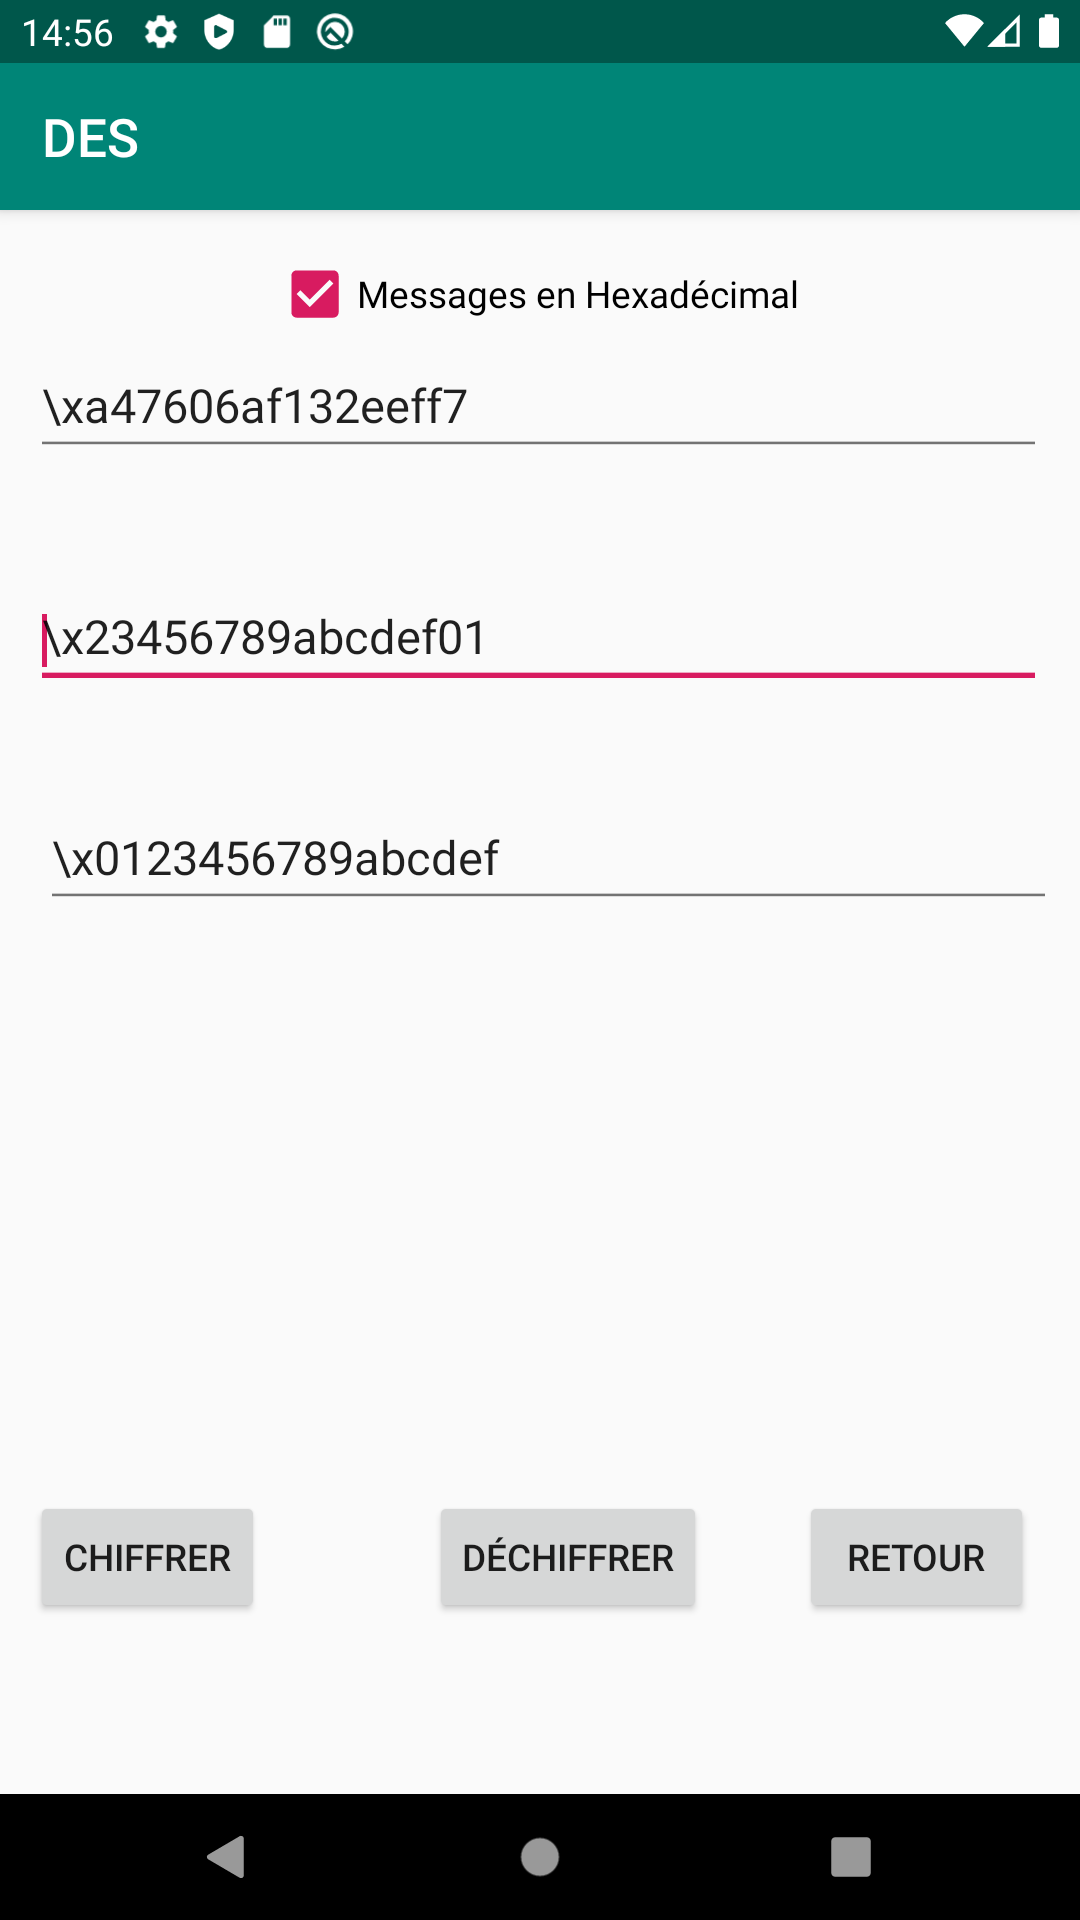
\includegraphics[width=.35\linewidth]{./img/des_d_hexa.png} \\
      Chiffrage de "\textbackslash x23456789abcdef01" avec la clé "\textbackslash x0123456789abcdef" & Déchiffrage \\
    \end{tabular}
    \caption{Chiffrage et déchiffrage en hexadécimal avec le \textbf{DES}}\label{fig:des_hex}
\end{figure}

\begin{figure}[b!]
    \centering
    \begin{tabular}{cc}
      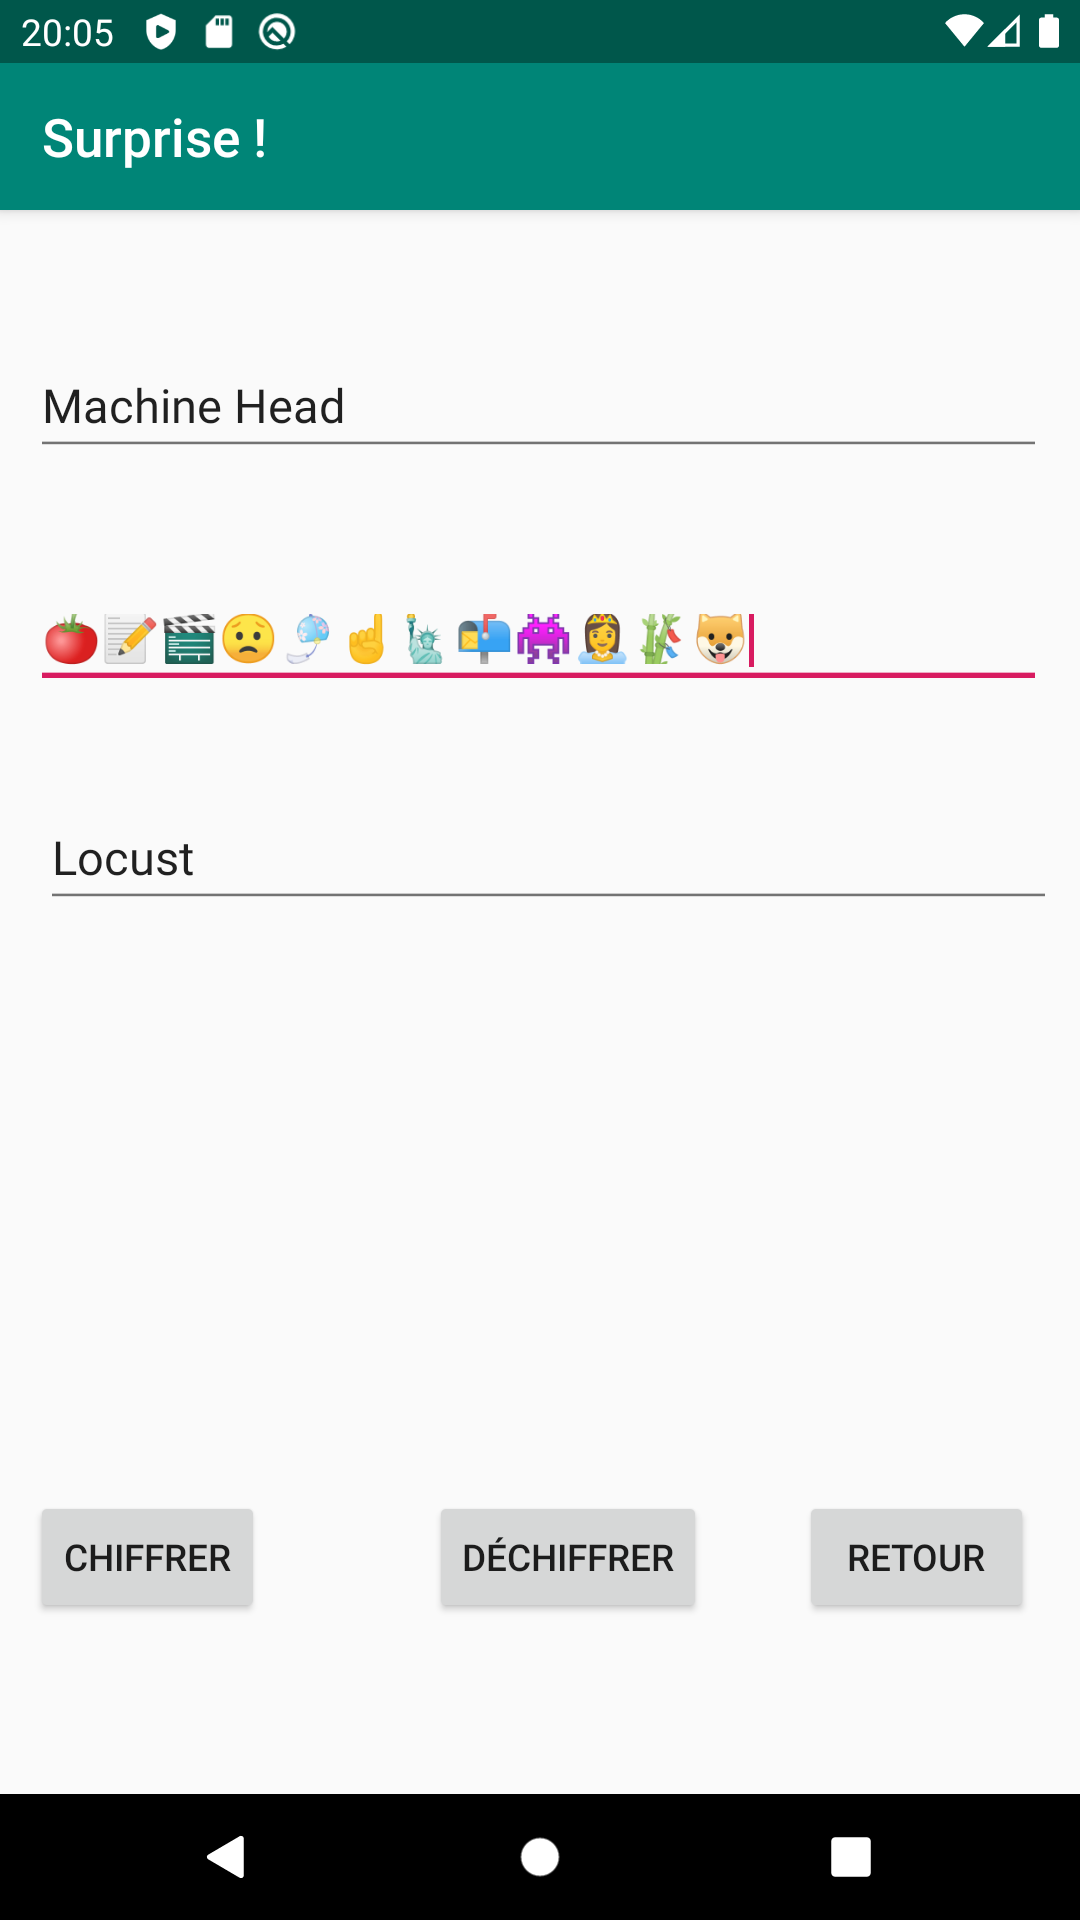
\includegraphics[width=.35\linewidth]{./img/surprise_e.png} &
      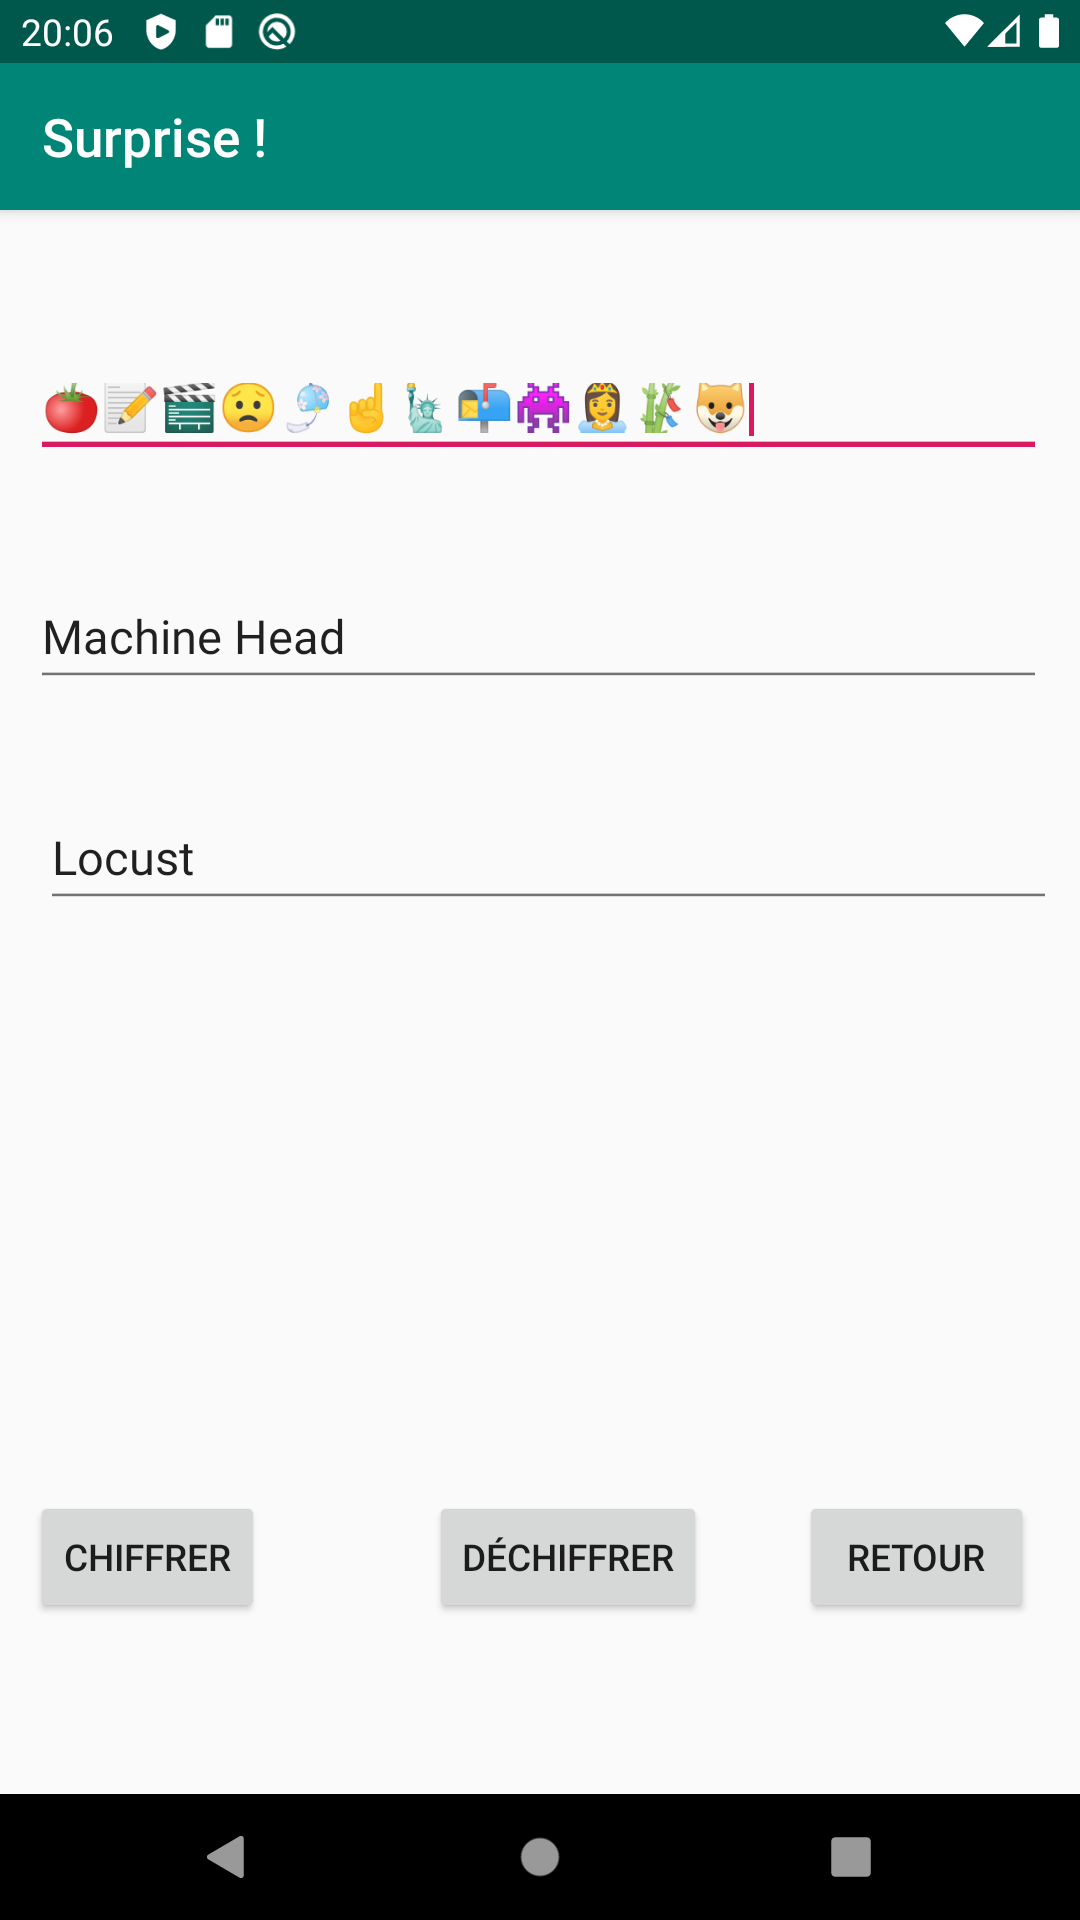
\includegraphics[width=.35\linewidth]{./img/surprise_d.png} \\
      Chiffrage de "Machine Head" avec la clé "Locust" & Déchiffrage \\
    \end{tabular}
    \caption{Chiffrage et déchiffrage avec un \textbf{algorithme surprise}}\label{fig:surprise}
\end{figure}

\begin{figure}[b!]
    \centering
    \begin{tabular}{cc}
      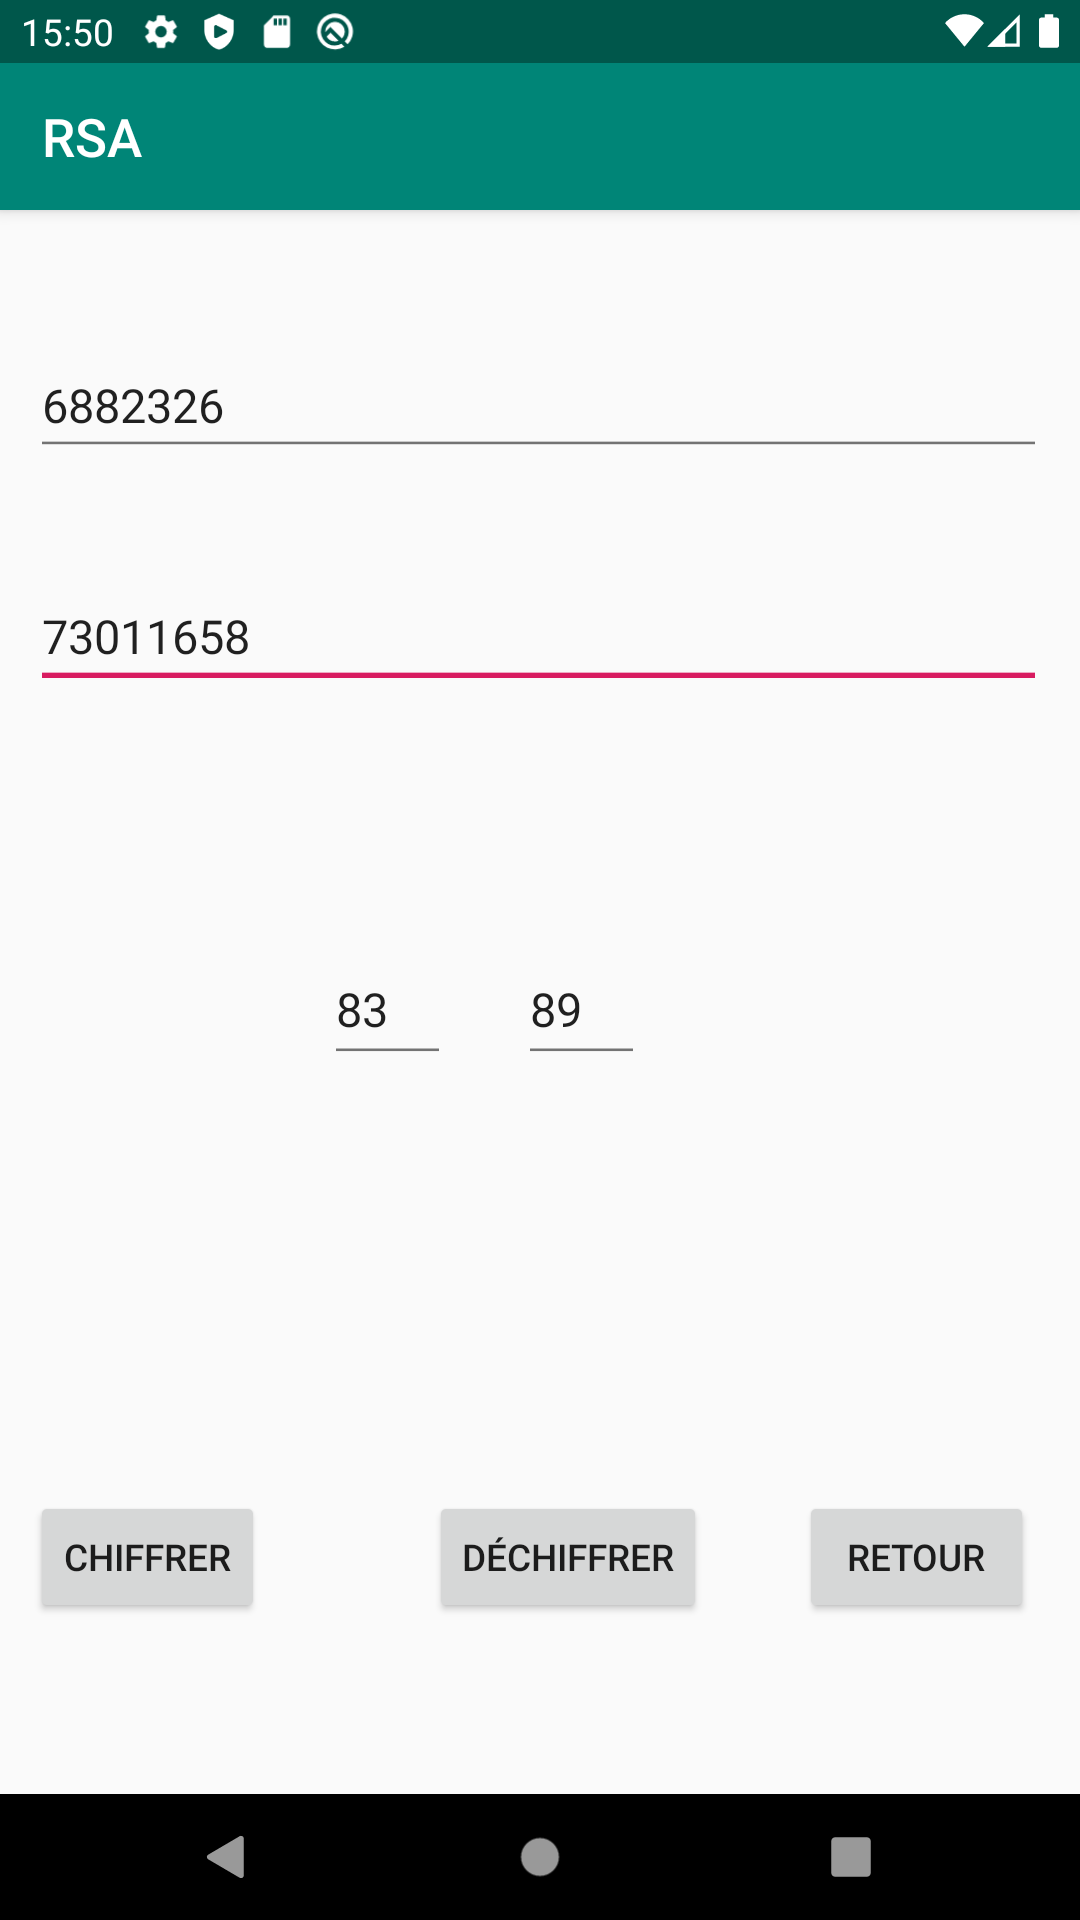
\includegraphics[width=.35\linewidth]{./img/RSA_e.png} &
      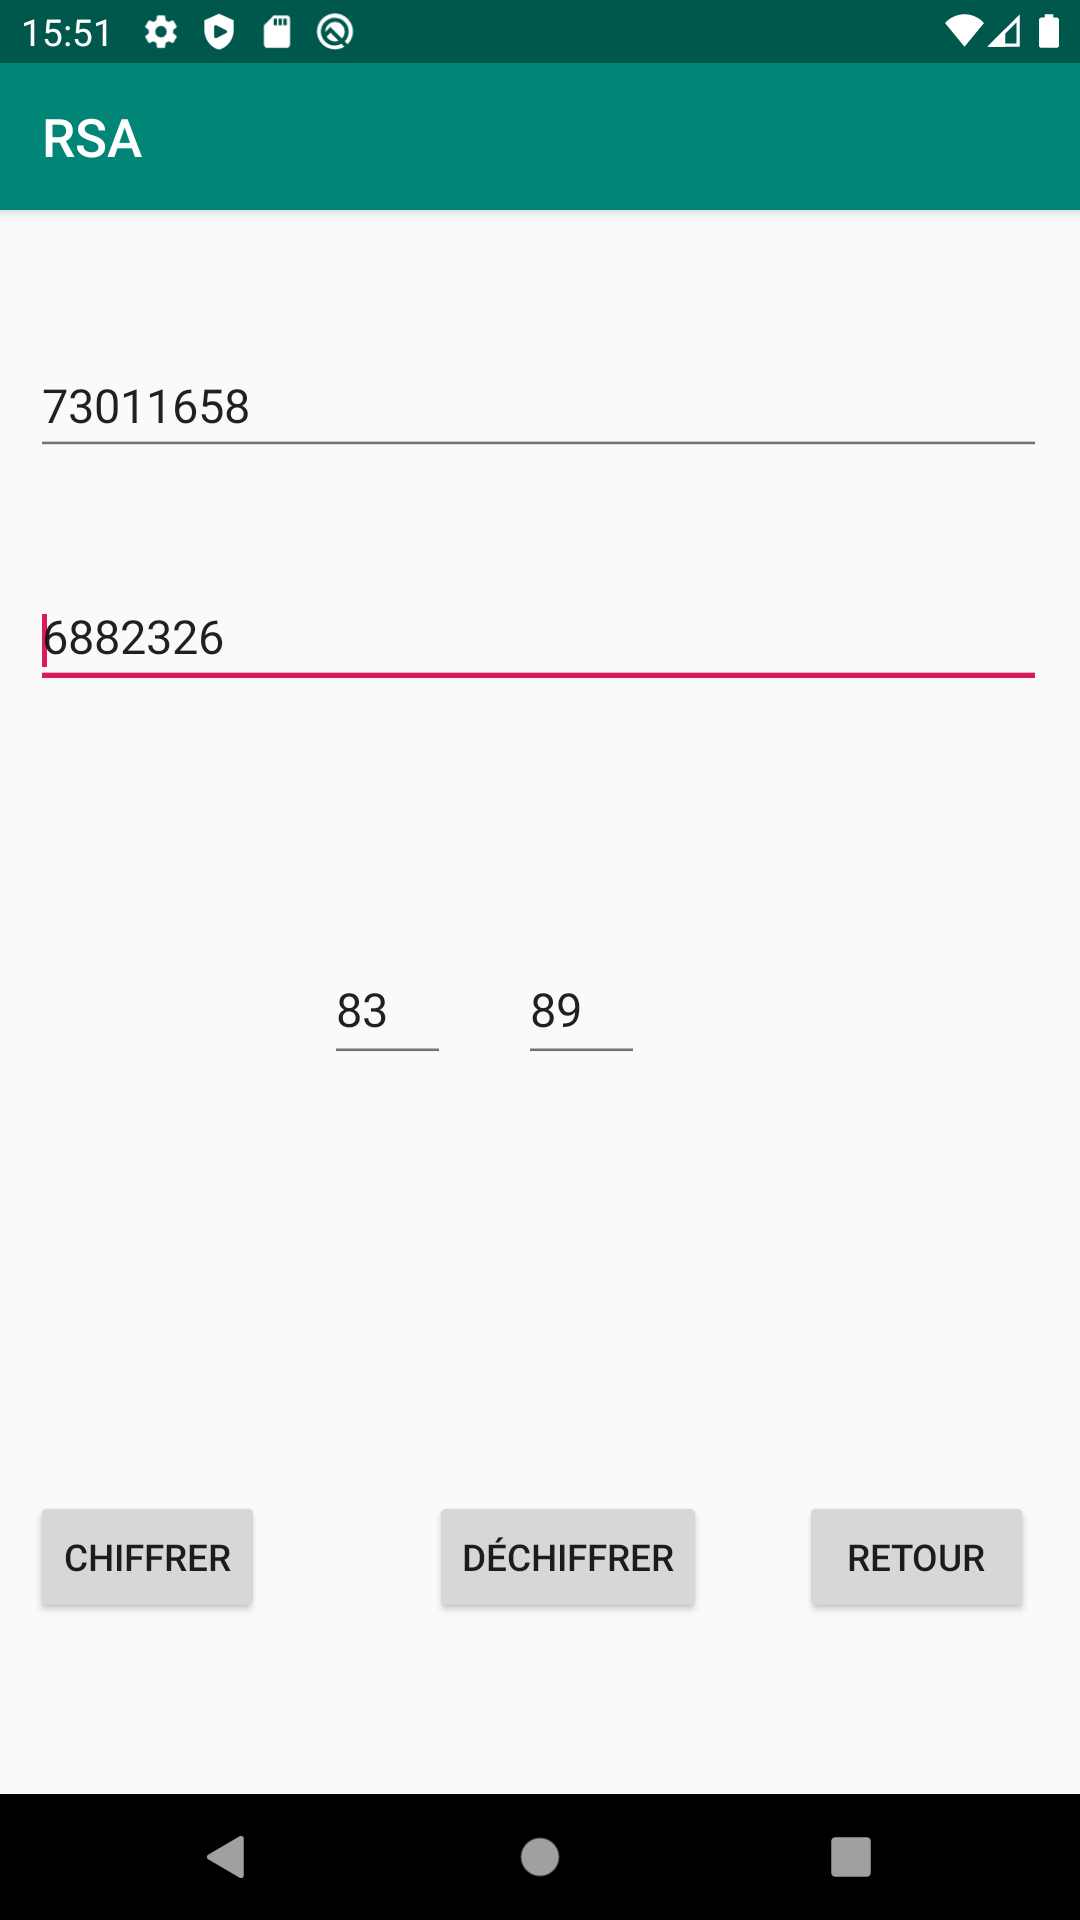
\includegraphics[width=.35\linewidth]{./img/RSA_d.png} \\
      Chiffrage de \textbf{6882326} pour $P=83$ et $Q=89$ & Déchiffrage \\
    \end{tabular}
    \caption{Chiffrage et déchiffrage avec un \textbf{algorithme surprise}}\label{fig:RSA}
\end{figure}

\bibliography{biblio}
\bibliographystyle{plain}

\nocite{*}


\end{document}